% Tikz plot for UQ. This is based on the tikz code of
% Fabian Schuh for the tikz examples website
\documentclass[10pt,final,xcolor=dvipsnames]{beamer}
%\usepackage{etex}

%\usetheme{Madrid}
%\usetheme{Boadilla}
\usetheme{default}
%\usetheme{seagull}
%\usetheme{Antibes}
\usecolortheme{dove}

\usepackage{xspace}
%\usepackage{enumitem}
\usepackage[mathscr]{euscript}
\usepackage{subcaption}
\hypersetup{colorlinks,linkcolor=,urlcolor=blue}

% \usetheme{Boadilla}
% \usecolortheme{seahorse}

% the macros, packages, etc:
\usepackage[absolute,overlay]{textpos}
\setbeamertemplate{items}[ball]
\setbeamertemplate{blocks}[rounded][shadow=true]
\setbeamertemplate{navigation symbols}{}
\newenvironment{reference}[2]{%
  \begin{textblock*}{\textwidth}(#1,#2)
  \scriptsize{\it\color{black}}}{\end{textblock*}}
\setbeamertemplate{blocks}[rounded]% [shadow=false]
\newenvironment{boxalertenv}{\begin{altenv}%
      {\usebeamertemplate{alerted text begin}\usebeamercolor[fg]{alerted text}\usebeamerfont{alerted text}\colorbox{bg}}
      {\usebeamertemplate{alerted text end}}{\color{.}}{}}{\end{altenv}}

\newcommand{\tcmag}[1]{\textcolor{magenta}{{#1}}}
\usepackage{graphicx}
\usepackage{multirow,color}
\usepackage{bbm}
\usepackage{amsfonts,amsmath,amssymb,amsbsy,amsthm}
\usepackage{movie15}
\usepackage{arydshln}

\makeatletter
\renewcommand*\env@matrix[1][*\c@MaxMatrixCols c]{%
  \hskip -\arraycolsep
  \let\@ifnextchar\new@ifnextchar
  \array{#1}}

%\usepackage{movie15}
%\usepackage{multimedia}
% custom commands (add your own macros here)

\definecolor{bronze}{rgb}{0.8, 0.5, 0.2}
\definecolor{goldenyellow}{rgb}{1.0, 0.87, 0.0}
\definecolor{amber}{rgb}{1.0, 0.75, 0.0}
\definecolor{azure}{rgb}{0.94, 1.0, 1.0}
\definecolor{bittersweet}{rgb}{1.0, 0.44, 0.37}
\definecolor{brass}{rgb}{0.71, 0.65, 0.26}
\definecolor{camel}{rgb}{0.76, 0.6, 0.42}
\setbeamercolor{block body}{bg=camel!30}
\usefonttheme[onlymath]{serif}
\usepackage{color}

\usepackage{amsmath}
\usepackage{mathtools}
\usepackage{tikz}
\usepackage{amsfonts,amsmath,amssymb,amsbsy,amsthm}
%\usecolortheme{tango}

%\usefonttheme{serif}     % Font theme: serif
%\usefonttheme[stillsansseriftext]{serif} 
%\renewcommand*\familydefault{\sfdefault}

\usepackage{pgf}
%\usepackage{pgfplots}
\usepackage{amssymb}
\usepackage{amsmath}
\usepackage{tikz}
\usepackage{verbatim}
%\usepackage{movie15}
\usepackage{tikz,pgfplots}

%\usepackage[active,tightpage]{preview}
%\PreviewEnvironment{tikzpicture}
\usetikzlibrary{arrows,automata}
\usetikzlibrary{positioning}
\usetikzlibrary{fit}

%\input{ccgodef}
\newcommand{\iparb}{\bar{\ipar}}
\newcommand{\euclidnorm}[1]{\left\| {#1} \right\|_2}
\newcommand{\incu}{\upupsilon}
\newcommand{\incp}{\uprho}
\newcommand{\QoIquad}{\QoI_\text{quad}}
\newcommand{\tcblue}[1]{\textcolor{blue}{#1}}

%%%%%%%%%%%%%%%%%%%%%%%%%%%%%%%%%%%%%%%%%%%%%%%%%%%%%%
%% this def file is based on the ccgodef
%%%%%%%%%%%%%%%%%%%%%%%%%%%%%%%%%%%%%%%%%%%%%%%%%%%%%
% packages
%\usepackage{booktabs}
%\usepackage[mathscr]{euscript}
%\usepackage{color}
%% mathdesgin or ams
%%\usepackage{amssymb,mathrsfs}
%\usepackage{graphicx}
%\usepackage{algorithmic,algorithm}
%\usepackage{tikz,pgfplots}
%\usepackage{upgreek}
%%\usepackage{showkeys,cite}
%\usepackage{multirow}
%\usepackage{yfonts}
%\usepackage{mathtools}
%\usepackage[normalem]{ulem}
%\usepackage{latexsym}
%\usepackage{url}
%\usepackage{amsmath,amssymb,amsbsy,amsfonts}
%\usepackage{enumitem}

\newcommand{\zapspace}{\topsep=0pt\partopsep=0pt\itemsep=0pt\parskip=0pt}

%% Notice macros
%\newcommand{\notice}[1]{\textcolor{Chameleon3}{#1}}
%\newcommand{\Notice}[1]{\textcolor{ScarletRed2}{#1}}
%\newcommand{\nnote}[1]{\noindent\emph{\textcolor{grass}{N: #1\,}}}
%\newcommand{\unote}[1]{\noindent\emph{\textcolor{blue}{U: #1\,}}}
%\newcommand{\onote}[1]{\noindent\emph{\textcolor{red}{O: #1\,}}}
%
%% colors
%\definecolor{utorange}{rgb}{0.8,0.33,0.}
%\definecolor{themec}{RGB}{51,108,121}
%\definecolor{darkred}{rgb}{.6,.1,.1}
%\definecolor{darkblue}{rgb}{.1,.1,.9}
%\definecolor{greenback}{rgb}{.19,.94,.13}
%\definecolor{orange}{rgb}{.76,.39,.13}
%\definecolor{grass}{rgb}{.19,.64,.13}
%\definecolor{sierp}{RGB}{209,28,209}
%\definecolor{bgorange}{rgb}{1.,.95,.78}
%\definecolor{grassgreen}{RGB}{92,135,39}
%\definecolor{thinbox}{rgb}{.7,.8,1.}

% general
\newcommand{\defeq}{\vcentcolon=}
%\newcommand{\del}[2]{\frac{\partial{#1}}{\partial{#2}}}
\renewcommand{\vec}[1]{{\mathchoice
                     {\mbox{\boldmath$\displaystyle{#1}$}}
                     {\mbox{\boldmath$\textstyle{#1}$}}
                     {\mbox{\boldmath$\scriptstyle{#1}$}}
                     {\mbox{\boldmath$\scriptscriptstyle{#1}$}}}}
\renewcommand{\ker}{\mathsf{ker}}
\newcommand{\ran}{\mathsf{range}}
\newcommand{\dom}{\mathsf{dom}}
\newcommand{\trace}{\mathsf{tr}}
\newcommand{\eps}{\varepsilon}
%\newcommand{\norm}[1]{\left\| {#1} \right\|}
\newcommand{\ip}[2]{{\left\langle {#1}, {#2} \right\rangle}}
\newcommand{\mip}[2]{\left\langle{#1}, {#2}\right\rangle_{\!\scriptscriptstyle{\text{M}}}}
\newcommand{\mat}[1]{\mathbf{{#1}}}
\newcommand\restr[2]{{
  \left.\kern-\nulldelimiterspace % automatically resize the bar with \right
  {#1}\vphantom{\big|} \right|_{#2}}}
\newcommand{\angles}[1]{\left\langle #1 \right\rangle}

% sets of numbers
\newcommand{\R}{\mathbb{R}}
\newcommand{\Z}{\mathbb{Z}}
\newcommand{\N}{\mathbb{N}}

\newcommand{\BB}{\mat{B}}
\newcommand{\Amat}{\mat{A}}
\newcommand{\VV}{\mat{V}}
\newcommand{\RR}{\mat{R}}

% commonly used mathcals
\newcommand{\A}{\mathcal{A}}
\newcommand{\B}{\mathcal{B}}
\newcommand{\C}{\mathcal{C}}
\newcommand{\D}{\mathcal{D}}
\newcommand{\E}{\mathcal{E}}
\newcommand{\F}{\mathcal{F}}
\newcommand{\G}{\mathcal{G}}
\newcommand{\J}{\mathcal{J}}
\newcommand{\U}{\mathcal{U}}
\newcommand{\Reg}{\mathcal{R}}

% shorthands
\newcommand{\bit}{\begin{itemize}}
\newcommand{\eit}{\end{itemize}}
\newcommand{\bdm} {\begin{displaymath}}
\newcommand{\edm} {\end{displaymath}}

% Probability (general)
\newcommand{\prob}{\mathsf{Prob}}
\newcommand{\borel}{\mathscr{B}}
\newcommand{\ave}{\mathsf{E}}
\newcommand{\GM}[2]{\mathcal{N}\!\left( {#1}, {#2}\right)}

% Bayesian stuff

\newcommand{\noisem}{\mu_{\text{noise}}}
\newcommand{\obs}{\vec{d}}
\newcommand{\ipar}{m}

\newcommand{\iparpr}{m_{\text{pr}}}
\newcommand{\iparref}{m_{\text{ref}}}
\newcommand{\iparmap}{m_{\scriptscriptstyle\text{MAP}}}
\newcommand{\dpar}{\vec{m}}
\newcommand{\dparmap}{\vec{m}_{\scriptscriptstyle\text{MAP}}}
%\newcommand{\priorm}{\mu_{\text{pr}}}
%\newcommand{\postm}{\mu_{\text{post}}}
\newcommand{\M}{\mat{M}}% the Mass matrix
%\newcommand{\ff}{\vec{f}}     % parameter-to-obs MAP
\newcommand{\ff}{\mathcal{F}} % parameter-to-obs MAP
\newcommand{\aff}{\tilde{\mathcal{F}}} % parameter-to-obs MAP
\newcommand{\noise}{\bs e}
\newcommand{\observables}{\bs d}
\newcommand{\data}{ \observables_{\rm{obs}} }
\newcommand{\uobs}{ \uu_{\rm{obs}} }
\newcommand{\datacomponent}[1]{ \observables_{\rm{obs}}^{#1} }
\newcommand{\FF}{{\ensuremath{\mat{F}}}}
\newcommand{\W}{{\ensuremath{\mat{W}}}}
\newcommand{\I}{{\ensuremath{\mat{I}}}}

\newcommand{\prior} {\pi_{\mbox{\tiny prior}}}
\newcommand{\like}{\pi_{\mbox{\tiny like}}}
\newcommand{\piobs}{\pi_{\mbox{\tiny obs}}}
\newcommand{\post}{\pi_{\mbox{\tiny post}}}
\newcommand{\pinoise}{\pi_{\mbox{\tiny noise}}}

\newcommand{\mupost}{\mu_{\mbox{\tiny post}}}
\newcommand{\muprior}{\mu_{\mbox{\tiny prior}}}

\newcommand{\ncov} {\bs{\Gamma}_{\!\mbox{\tiny noise}} }
\newcommand{\prcov} {\bs{\Gamma}_{\!\mbox{\tiny prior}} }
\newcommand{\postcov} {\bs{\Gamma}_{\!\mbox{\tiny post}} }
\newcommand{\aFF}{{\tilde{\ensuremath{\mat{F}}}}}
\newcommand{\ncovw} {\bs{W}}
\newcommand{\prcovr} {\bs{R}}

\newcommand{\Cprior}{\mathcal{C}_{\text{\tiny{prior}}}}
\newcommand{\Cpost}{\mathcal{C}_{\text{\tiny{post}}}}

\newcommand{\map} {{m}_{\mbox{\tiny MAP}} }
\newcommand{\dmap} {{\vec{m}}_{\mbox{\tiny MAP}} }
\newcommand{\mpr} {{\vec{m}}_{\mbox{\tiny pr}} }
\newcommand{\dbeta}{\vec{\beta}}
\newcommand{\dn}{\vec{n}}



\newcommand{\Hpost}  { \bs H }
\newcommand{\Hmisfit}{ \mat{H}_{\mbox{\tiny misfit}} }
\newcommand{\tHmisfit}{\tilde{\mat{H}}_{\mbox{\tiny misfit}} }
\newcommand{\HT}{\matrix{\tilde{H}}_{\mbox{\tiny misfit}}}
\newcommand{\HTinf}{\tilde{H}_{\text{misfit}}}
\newcommand{\Vr} {\bs V_r}
\newcommand{\Dr} {\bs D_r}
\newcommand{\Ir} {\bs I_r}

%\newcommand{\Ge}{ \ensuremath{\matrix{G}}_{\!\mbox{\tiny e}}}
%\newcommand{\Op}{ \ensuremath{\matrix{O}}_{\!\mbox{\tiny p}}}
\newcommand{\Ge}{ \mathcal{G}_{\!\mbox{\tiny e}}}
\newcommand{\Op}{ \mathcal{O}_{\!\mbox{\tiny p}}}
\newcommand{\HH}{ \ensuremath{\matrix{H}} }
\newcommand{\SI}{ \ensuremath{{\Sigma}} }
\newcommand{\PP}{ \ensuremath{\matrix{\Psi}} }
%\newcommand{\WW}{ \ensuremath{\matrix{W}} }
\newcommand{\WW}{ \mathcal{W}}

% Macros for three different forms of adjoint operator
\newcommand{\adjMacroMM}[1]{{#1}^*}
\newcommand{\adjMacroME}[1]{{#1}^\natural}
\newcommand{\adjMacroEM}[1]{{#1}^\diamond}
\newcommand{\adjMacroEMINV}[1]{{#1}^{-\diamond}}
\newcommand{\Aadj}{\adjMacroMM{\A}}
\newcommand{\Badj}{\adjMacroMM{\BB}}
\newcommand{\iFadj}{\adjMacroME{\iF}}
\newcommand{\Fadj}{\adjMacroME{\F}}
\newcommand{\Vadj}{\adjMacroEM{\VV}}
\newcommand{\Ladj}{\adjMacroEM{\L}}

\def\bfG{\mbox{\boldmath$G$}}
\newcommand{\mc}[1]{\mathcal{#1}}

%%%%%%%%%%%%%%%%%%%%%%%%%%%%%%%%%%%%
% custom commands to the sc14 paper
%%%%%%%%%%%%%%%%%%%%%%%%%%%%%%%%%%%%
\newcommand{\SNR}{\ensuremath{\text{SNR}}}

\newcommand{\gbf}[1]{\boldsymbol{#1}}
\newcommand{\bs}[1]{\ensuremath{\boldsymbol{#1}}}

\newcommand{\edot}{\dot{\gbf{\varepsilon}}}
\newcommand{\edotsec}{\edot_\mathrm{II}}
\newcommand{\secinve}{\edot_\mathrm{II}}

\DeclareMathOperator{\sym}{sym}
%\DeclareMathOperator{\trace}{tr}
%\DeclareMathOperator{\diag}{diag}

\newcommand{\Div}{\mbox{div}}
\newcommand{\Grad}{{\bf \nabla}}
\newcommand{\grad}{\nabla}

\newcommand{\pt}{\tilde{p}}
\newcommand{\vt}{\tilde{\vv}}
\newcommand{\qt}{\tilde{q}}
\newcommand{\betat}{\tilde{\beta}}

\newcommand{\uh}{\hat{\uu}}
\newcommand{\ph}{\hat{p}}
\newcommand{\vh}{\hat{\vv}}
\newcommand{\qh}{\hat{q}}
\newcommand{\betah}{\hat{\beta}}

\renewcommand{\vec}[1]{\gbf{#1}}
\newcommand{\cvec}[1]{{#1}}

\newcommand{\uu}{\ensuremath{\vec{u}}}
\newcommand{\vv}{\ensuremath{\vec{v}}}

\definecolor{darkblue}{rgb}{.1,.1,.9}
\definecolor{utorange}{rgb}{0.8,0.33,0.}
% this are only needed for presentations
\newcommand{\tcb}[1]{\textcolor{blue}{{#1}}}
\newcommand{\tcdb}[1]{\textcolor{utorange}{{#1}}}
\newcommand{\tcr}[1]{\ensuremath{\textcolor{red}{{#1}}}}
\newcommand{\tcdr}[1]{\textcolor{darkred}{{#1}}}
\newcommand{\tcm}[1]{\textcolor{ForestGreen}{{#1}}}
\newcommand{\tcmag}[1]{\textcolor{magenta}{{#1}}}
\newcommand{\tco}[1]{\textcolor{VioletRed}{{#1}}}
\newcommand{\tcc}[1]{\textcolor{cyan}{{#1}}}
\newcommand{\dg}[1]{\textcolor{black!65!green}{{#1}}}
\newcommand{\tcg}[1]{\textcolor{blue!70!black!30!green}{{#1}}}
\newcommand{\tcdg}[1]{\textcolor{blue!20!black!50!green}{{#1}}}
\newcommand{\tcch}[1]{\textcolor{cyan}{\hat{{#1}}}}
\newcommand{\tcmhb}[1]{\textcolor{magenta}{\hat{\gbf{{#1}}}}}
\newcommand{\tcmh}[1]{\textcolor{magenta}{\hat{{#1}}}}
\newcommand{\tcbb}[1]{\textcolor{blue}{\gbf{{#1}}}}
\newcommand{\tcgb}[1]{\textcolor{grass}{\gbf{{#1}}}}
\newcommand{\tcct}[1]{\textcolor{cyan}{\tilde{{#1}}}}
\newcommand{\tcmtb}[1]{\textcolor{magenta}{\tilde{\gbf{{#1}}}}}
\newcommand{\tcmt}[1]{\textcolor{magenta}{\tilde{{#1}}}}
\newcommand{\tcotb}[1]{\textcolor{utorange}{\tilde{\gbf{{#1}}}}}
\newcommand{\tcot}[1]{\textcolor{utorange}{\tilde{{#1}}}}
\newcommand{\tcohb}[1]{\textcolor{utorange}{\hat{\gbf{{#1}}}}}
\newcommand{\tcoh}[1]{\textcolor{utorange}{\hat{{#1}}}}

\renewcommand{\matrix}[1] {\ensuremath{\boldsymbol{#1}}}

\newcommand{\bndFS}{\Gamma_{\!\mbox{\scriptsize $FS$}}}
\newcommand{\bndB}{\Gamma_{\!\mbox{\scriptsize $B$}}}
\newcommand{\bndT}{\Gamma_{\!\mbox{\scriptsize $T$}}}

\usepackage{xspace}
\newcommand{\software}[1]{\texttt{#1}\xspace}
\newcommand{\hip}{\texttt{hIPPYlib}\xspace}
\newcommand{\bhip}{\texttt{{\bf hIPPYlib}}\xspace}
\newcommand{\Fe}{\texttt{FEniCS}\xspace}
\newcommand{\pet}{\texttt{PETSc}\xspace}


\newcommand{\del}{\partial}
%\newcommand{\D}{\mathcal{D}}
\newcommand{\Ns}{{N_s}}
\newcommand{\Ntau}{{N_{\tau}}}
\newcommand{\iFF}{\mathcal{F}}
%\newcommand{\priorm}{\muprior}
\newcommand{\Acal}{\mc{A}}
%\newcommand{\postm}{\mupost}
\newcommand{\iparpost}{\ipar_\text{post}}
\newcommand{\dd}{\vec{\bar{d}}}
\newcommand{\obsop}{\mathcal{B}}

\newcommand{\GN}{\ensuremath{\Gamma_{\!\!N}}}
\newcommand{\Exp}[1]{e^{{#1}}}
\newcommand{\GD}{\ensuremath{\Gamma_{\!\!D}}}
\newcommand{\Vg}{\mathscr{V}_{\!g}}
\newcommand{\V}{\mathscr{V}_{\!\scriptscriptstyle{0}}}
\newcommand{\eip}[2]{\left\langle{#1}, {#2}\right\rangle_{\!{\R^q}}}
\newcommand{\Wn}{\mat{W}_{\!\sigma}}
\newcommand{\cip}[2]{\left\langle{#1}, {#2}\right\rangle_{\!\CM}}
\newcommand{\CM}{\mathscr{E}}
\newcommand{\LI}{\mathscr{L}}
\renewcommand{\H}{\mathcal{H}}
\newcommand{\Nd}{{n_{\text{d}}}}
\newcommand{\Ntr}{{n_{\text{tr}}}}
\newcommand{\ipart}{m_{\scriptscriptstyle\text{true}}}
\newcommand{\ut}[1]{\ensuremath{\tilde{#1}}}

\newcommand{\LRp}[1]{\left( #1 \right)}
\newcommand{\LRs}[1]{\left[ #1 \right]}
\newcommand{\LRa}[1]{\left< #1 \right>}
\newcommand{\LRc}[1]{\left\{ #1 \right\}}

\newcommand{\xx}{\ensuremath{\boldsymbol x}}
\newcommand{\rr}{\ensuremath{\boldsymbol r}}
\newcommand{\e}{\ensuremath{\boldsymbol e}}
\newcommand{\x}{\xx}
\newcommand{\y}{\ensuremath{\boldsymbol y}}
\newcommand{\z}{\ensuremath{\boldsymbol z}}
\renewcommand{\r}{\ensuremath{\boldsymbol r}}
\newcommand{\s}{\ensuremath{\boldsymbol s}}

\newcommand{\hilb}{\mathscr{H}}
\newcommand{\half} {\ensuremath{\frac{1}{2}}}
\newcommand{\nor}[1]{\left\| #1 \right\|}
\newcommand{\equaldef}{{:=}}
\newcommand{\iFFadj}{\adjMacroMM{\iFF}}

\newcommand{\istate}{u}
\newcommand{\iparspace}{\mathcal{M}}
\newcommand{\iadj}{p}
\DeclareMathOperator*{\argmin}{argmin} 
\DeclareMathOperator{\diag}{diag} 


\newcommand{\err}{\vec{\eta}}
\newcommand{\beps}{\bs{\eps}}
\newcommand{\bbeps}{\bar{\bs{\eps}}}
\newcommand{\bnu}{\bs{\nu}}
\newcommand{\ncovbeps} {\bs{\Gamma}_{\!\mbox{\tiny \beps}} }
\newcommand{\ncovbnu} {\bs{\Gamma}_{\!\mbox{\tiny \bnu}} }
\newcommand{\norm}[2][]{\left\Vert #2\right\Vert_{#1}}
\newcommand{\dbetamap}{\vec{\beta}_{\scriptscriptstyle\text{MAP}}}
\newcommand{\betamap}{{\beta}_{\scriptscriptstyle\text{MAP}}}
\newcommand{\smallB}{\scriptscriptstyle\text{B}}
\definecolor{lightblue}{cmyk}{0.88,0.44,0,0.07}
\newcommand{\betapr}{\beta_{\text{pr}}}
\newcommand{\ntrue}{a_{\scriptscriptstyle\text{true}}}
\newcommand{\NoiseForcing}{\xi}
\newcommand{\ProbMeasClass}{\mathcal{P}}
\newcommand{\ProbMeas}{\mathbbm{P}}
\newcommand{\SigmaAlg}{F}

\newcommand{\Hmatrix}{\bs{H}}

\tikzset{
    state/.style={
           rectangle,
           rounded corners,
           draw=black, very thick,
           minimum height=3em,
           inner sep=1pt,
           text centered,
           },
}

%
\newcommand{\zapspace}{\topsep=0pt\partopsep=0pt\itemsep=0pt\parskip=0pt}

%
\newcommand{\notice}[1]{\textcolor{Chameleon3}{#1}}
\newcommand{\Notice}[1]{\textcolor{ScarletRed2}{#1}}
\newcommand{\nnote}[1]{\noindent\emph{\textcolor{grass}{N: #1\,}}}
\newcommand{\emil}[1]{\noindent\emph{\textcolor{blue}{Emil: #1\,}}}
\newcommand{\julie}[1]{\noindent\emph{\textcolor{red}{Julie: #1\,}}}
\newcommand{\unote}[1]{\noindent\emph{\textcolor{blue}{U: #1\,}}}
\newcommand{\onote}[1]{\noindent\emph{\textcolor{red}{O: #1\,}}}
\definecolor{mygreen}{rgb}{0.5,0.05,0.15}
\newcommand{\cosmin}[1]{\noindent\emph{\textcolor{mygreen}{#1\,}}}

%
\definecolor{utorange}{rgb}{0.8,0.33,0.}
\definecolor{themec}{RGB}{51,108,121}
\definecolor{darkred}{rgb}{.6,.1,.1}
\definecolor{darkblue}{rgb}{.1,.1,.9}
\definecolor{greenback}{rgb}{.19,.94,.13}
\definecolor{orange}{rgb}{.76,.39,.13}
\definecolor{grass}{rgb}{.19,.64,.13}
\definecolor{sierp}{RGB}{209,28,209}
\definecolor{bgorange}{rgb}{1.,.95,.78}
\definecolor{grassgreen}{RGB}{92,135,39}
\definecolor{thinbox}{rgb}{.7,.8,1.}

%
\newcommand{\defeq}{\vcentcolon=}
%
\renewcommand{\vec}[1]{{\mathchoice
                     {\mbox{\boldmath$\displaystyle{#1}$}}
                     {\mbox{\boldmath$\textstyle{#1}$}}
                     {\mbox{\boldmath$\scriptstyle{#1}$}}
                     {\mbox{\boldmath$\scriptscriptstyle{#1}$}}}}
\renewcommand{\ker}{\mathsf{ker}}
\newcommand{\ran}{\mathsf{range}}
\newcommand{\dom}{\mathsf{dom}}
\newcommand{\trace}{\mathsf{tr}}
\newcommand{\eps}{\varepsilon}
\newcommand{\norm}[1]{\left\| {#1} \right\|}
\newcommand{\ip}[2]{{\left\langle {#1}, {#2} \right\rangle}}
\newcommand{\mip}[2]{\left\langle{#1}, {#2}\right\rangle_{\!\scriptscriptstyle{\text{M}}}}
\newcommand{\mat}[1]{\mathbf{{#1}}}
\newcommand\restr[2]{{
  \left.\kern-\nulldelimiterspace %
  {#1}\vphantom{\big|} \right|_{#2}}}
\newcommand{\angles}[1]{\left\langle #1 \right\rangle}

%
\newcommand{\R}{\mathbb{R}}
\newcommand{\Z}{\mathbb{Z}}
\newcommand{\N}{\mathbb{N}}

\newcommand{\BB}{\mat{B}}
\newcommand{\Amat}{\mat{A}}
\newcommand{\VV}{\mat{V}}
\newcommand{\RR}{\mat{R}}

%
\newcommand{\A}{\mathcal{A}}
\newcommand{\B}{\mathcal{B}}
\newcommand{\C}{\mathcal{C}}
\newcommand{\D}{\mathcal{D}}
\newcommand{\E}{\mathcal{E}}
\newcommand{\F}{\mathcal{F}}
\newcommand{\G}{\mathcal{G}}
\newcommand{\J}{\mathcal{J}}
\newcommand{\U}{\mathcal{U}}
\newcommand{\Reg}{\mathcal{R}}

%
\newcommand{\bit}{\begin{itemize}}
\newcommand{\eit}{\end{itemize}}
\newcommand{\bdm} {\begin{displaymath}}
\newcommand{\edm} {\end{displaymath}}

%
\newcommand{\prob}{\mathsf{Prob}}
\newcommand{\borel}{\mathscr{B}}
\newcommand{\ProbMeasClass}{\mathcal{P}}
\newcommand{\ProbMeas}{\mathbbm{P}}
\newcommand{\SigmaAlg}{F}
\newcommand{\ave}{\mathsf{E}}
\newcommand{\GM}[2]{\mathcal{N}\!\left( {#1}, {#2}\right)}

%
\newcommand{\NoiseForcing}{\xi}
\newcommand{\noisem}{\mu_{\text{noise}}}
\newcommand{\obs}{\F}%
\newcommand{\dobs}{{\vec{d}}}
\newcommand{\obsT}{{\vec{d}_{\scriptscriptstyle\text{obs}}}}
\newcommand{\ipar}{m}
\newcommand{\iparT}{m_{\mathrm T}}
\newcommand{\iparpr}{m_{\text{prior}}}
\newcommand{\iparmap}{m_{\scriptscriptstyle\text{MAP}}}
\newcommand{\dpar}{\vec{m}}
\newcommand{\dparmap}{\vec{m}_{\scriptscriptstyle\text{MAP}}}
%
%
\newcommand{\M}{\mat{M}}%
%
\newcommand{\ff}{\mathcal{F}} %
\newcommand{\noise}{\bs e}
\newcommand{\observables}{\bs d}
\newcommand{\data}{ \observables_{\rm{obs}} }
\newcommand{\uobs}{ \uu_{\rm{obs}} }
\newcommand{\datacomponent}[1]{ \observables_{\rm{obs}}^{#1} }
\newcommand{\FF}{{\ensuremath{\mat{F}}}}
\newcommand{\W}{{\ensuremath{\mat{W}}}}
\newcommand{\I}{{\ensuremath{\mat{I}}}}
\newcommand{\ScoreFcn}{S}
\newcommand{\Nobs}{M}
\newcommand{\Expectation}{\mathbb{E}}


\newcommand{\prior} {\pi_{\mbox{\tiny prior}}}
\newcommand{\like}{\pi_{\mbox{\tiny like}}}
\newcommand{\piobs}{\pi_{\mbox{\tiny obs}}}
\newcommand{\pinoise}{\pi_{\mbox{\tiny $\xi$}}}
\newcommand{\post}{\pi_{\mbox{\tiny post}}}

\newcommand{\mupost}{\mu_{\mbox{\tiny post}}}
\newcommand{\muprior}{\mu_{\mbox{\tiny prior}}}

\newcommand{\ncov} {\bs{\Gamma}_{\!\mbox{\tiny noise}} }
\newcommand{\prcov} {\bs{\Gamma}_{\!\mbox{\tiny prior}} }
\newcommand{\postcov} {\bs{\Gamma}_{\!\mbox{\tiny post}} }

\newcommand{\Cprior}{\mathcal{C}_{\text{\tiny{prior}}}}
\newcommand{\Cpost}{\mathcal{C}_{\text{\tiny{post}}}}

\newcommand{\map} {{m}_{\mbox{\tiny MAP}} }
\newcommand{\dmap} {{\vec{m}}_{\mbox{\tiny MAP}} }
\newcommand{\mpr} {{\vec{m}}_{\mbox{\tiny pr}} }
\newcommand{\dbeta}{\vec{m}}

\newcommand{\Hpost}  { \bs H }
\newcommand{\Hmisfit}{ \mat{H}_{\mbox{\tiny misfit}} }
\newcommand{\tHmisfit}{\tilde{\mat{H}}_{\mbox{\tiny misfit}} }
\newcommand{\HT}{\matrix{\tilde{H}}_{\mbox{\tiny misfit}}}
\newcommand{\HTinf}{\tilde{H}_{\text{misfit}}}
\newcommand{\Vr} {\bs V_r}
\newcommand{\Dr} {\bs D_r}
\newcommand{\Ir} {\bs I_r}

%
%
\newcommand{\Ge}{ \mathcal{G}_{\!\mbox{\tiny e}}}
\newcommand{\Op}{ \mathcal{O}_{\!\mbox{\tiny p}}}
\newcommand{\HH}{ \ensuremath{\matrix{H}} }
\newcommand{\SI}{ \ensuremath{{\Sigma}} }
\newcommand{\PP}{ \ensuremath{\matrix{\Psi}} }
%
\newcommand{\WW}{ \mathcal{W}}

%
\newcommand{\adjMacroMM}[1]{{#1}^*}
\newcommand{\adjMacroME}[1]{{#1}^\natural}
\newcommand{\adjMacroEM}[1]{{#1}^\diamond}
\newcommand{\adjMacroEMINV}[1]{{#1}^{-\diamond}}
\newcommand{\Aadj}{\adjMacroMM{\A}}
\newcommand{\Badj}{\adjMacroMM{\BB}}
\newcommand{\iFadj}{\adjMacroME{\iF}}
\newcommand{\Fadj}{\adjMacroME{\F}}
\newcommand{\Vadj}{\adjMacroEM{\VV}}
\newcommand{\Ladj}{\adjMacroEM{\L}}

\def\bfG{\mbox{\boldmath$G$}}
\newcommand{\mc}[1]{\mathcal{#1}}

%
%
%
\newcommand{\SNR}{\ensuremath{\text{SNR}}}

\newcommand{\gbf}[1]{\boldsymbol{#1}}
\newcommand{\bs}[1]{\ensuremath{\boldsymbol{#1}}}

\newcommand{\edot}{\dot{\gbf{\varepsilon}}}
\newcommand{\edotsec}{\edot_\mathrm{II}}
\newcommand{\secinve}{\edot_\mathrm{II}}

\DeclareMathOperator{\sym}{sym}
%
%

\newcommand{\Div}{\mbox{div}}
\newcommand{\Grad}{{\bf \nabla}}

\newcommand{\pt}{\tilde{p}}
\newcommand{\vt}{\tilde{\vv}}
\newcommand{\qt}{\tilde{q}}
\newcommand{\betat}{\tilde{\beta}}

\newcommand{\uh}{\hat{\uu}}
\newcommand{\ph}{\hat{p}}
\newcommand{\vh}{\hat{\vv}}
\newcommand{\qh}{\hat{q}}
\newcommand{\betah}{\hat{\beta}}

\newcommand{\permeab}{\mathrm{m}}

\renewcommand{\vec}[1]{\gbf{#1}}
\newcommand{\cvec}[1]{{#1}}

\newcommand{\uu}{\ensuremath{\vec{u}}}
\newcommand{\vv}{\ensuremath{\vec{v}}}

\newcommand{\tcb}[1]{\textcolor{blue}{{#1}}}
\newcommand{\tcdb}[1]{\textcolor{darkblue}{{#1}}}
\newcommand{\tcr}[1]{\ensuremath{\textcolor{red}{{#1}}}}
\newcommand{\tcdr}[1]{\textcolor{darkred}{{#1}}}
\newcommand{\tcm}[1]{\textcolor{ForestGreen}{{#1}}}
\newcommand{\tco}[1]{\textcolor{VioletRed}{{#1}}}
\newcommand{\tcc}[1]{\textcolor{cyan}{{#1}}}
\newcommand{\dg}[1]{\textcolor{black!65!green}{{#1}}}
\newcommand{\tcg}[1]{\textcolor{blue!70!black!30!green}{{#1}}}
\newcommand{\tcdg}[1]{\textcolor{blue!20!black!50!green}{{#1}}}
\newcommand{\tcch}[1]{\textcolor{cyan}{\hat{{#1}}}}
\newcommand{\tcmhb}[1]{\textcolor{magenta}{\hat{\gbf{{#1}}}}}
\newcommand{\tcmh}[1]{\textcolor{magenta}{\hat{{#1}}}}
\newcommand{\tcbb}[1]{\textcolor{blue}{\gbf{{#1}}}}
\newcommand{\tcgb}[1]{\textcolor{grass}{\gbf{{#1}}}}
\newcommand{\tcct}[1]{\textcolor{cyan}{\tilde{{#1}}}}
\newcommand{\tcmtb}[1]{\textcolor{magenta}{\tilde{\gbf{{#1}}}}}
\newcommand{\tcmt}[1]{\textcolor{magenta}{\tilde{{#1}}}}
\newcommand{\tcotb}[1]{\textcolor{utorange}{\tilde{\gbf{{#1}}}}}
\newcommand{\tcot}[1]{\textcolor{utorange}{\tilde{{#1}}}}
\newcommand{\tcohb}[1]{\textcolor{utorange}{\hat{\gbf{{#1}}}}}
\newcommand{\tcoh}[1]{\textcolor{utorange}{\hat{{#1}}}}



\renewcommand{\matrix}[1] {\ensuremath{\boldsymbol{#1}}}

\newcommand{\bndFS}{\Gamma_{\!\mbox{\scriptsize $FS$}}}
\newcommand{\bndB}{\Gamma_{\!\mbox{\scriptsize $B$}}}
\newcommand{\bndT}{\Gamma_{\!\mbox{\scriptsize $T$}}}

\usepackage{xspace}
\newcommand{\software}[1]{\texttt{#1}\xspace}
\newcommand{\hip}{\texttt{hIPPYlib}\xspace}
\newcommand{\bhip}{\texttt{{\bf hIPPYlib}}\xspace}
\newcommand{\Fe}{\texttt{FEniCS}\xspace}
\newcommand{\pet}{\texttt{PETSc}\xspace}


\newcommand{\del}{\partial}
%
\newcommand{\Ns}{{N_s}}
\newcommand{\Ntau}{{N_{\tau}}}
\newcommand{\iFF}{\mathcal{F}}
%
\newcommand{\Acal}{\mc{A}}
%
\newcommand{\iparpost}{\ipar_\text{post}}
\newcommand{\dd}{\vec{\bar{d}}}
\newcommand{\obsop}{\mathcal{B}}

\newcommand{\GN}{\ensuremath{\Gamma_{\!\!N}}}
\newcommand{\Exp}[1]{e^{{#1}}}
\newcommand{\GD}{\ensuremath{\Gamma_{\!\!D}}}
\newcommand{\Vg}{\mathscr{V}_{\!g}}
\newcommand{\V}{\mathscr{V}_{\!\scriptscriptstyle{0}}}
\newcommand{\eip}[2]{\left\langle{#1}, {#2}\right\rangle_{\!{\R^q}}}
\newcommand{\Wn}{\mat{W}_{\!\sigma}}
\newcommand{\cip}[2]{\left\langle{#1}, {#2}\right\rangle_{\!\CM}}
\newcommand{\CM}{\mathscr{E}}
\newcommand{\LI}{\mathscr{L}}
\renewcommand{\H}{\mathcal{H}}
\newcommand{\Nd}{{n_{\text{d}}}}
\newcommand{\Ntr}{{n_{\text{tr}}}}
\newcommand{\ipart}{m_{\scriptscriptstyle\text{true}}}
\newcommand{\epsobs}{\varepsilon_{\scriptscriptstyle\text{obs}}}
\newcommand{\grad}{\nabla}
\newcommand{\ut}[1]{\ensuremath{\tilde{#1}}}

\newcommand{\LRp}[1]{\left( #1 \right)}
\newcommand{\LRs}[1]{\left[ #1 \right]}
\newcommand{\LRa}[1]{\left< #1 \right>}
\newcommand{\LRc}[1]{\left\{ #1 \right\}}

\newcommand{\xx}{\ensuremath{\boldsymbol x}}
\newcommand{\rr}{\ensuremath{\boldsymbol r}}
\newcommand{\e}{\ensuremath{\boldsymbol e}}
\newcommand{\x}{\xx}
\newcommand{\y}{\ensuremath{\boldsymbol y}}
\newcommand{\z}{\ensuremath{\boldsymbol z}}
\renewcommand{\r}{\ensuremath{\boldsymbol r}}
\newcommand{\s}{\ensuremath{\boldsymbol s}}

\newcommand{\hilb}{\mathscr{H}}
\newcommand{\half} {\ensuremath{\frac{1}{2}}}
\newcommand{\nor}[1]{\left\| #1 \right\|}
\newcommand{\equaldef}{{:=}}
\newcommand{\iFFadj}{\adjMacroMM{\iFF}}

\newcommand{\NEns}{{N_s}}
\newcommand{\ES}{{\mathrm{ES}}}

\newcommand{\CovFcn}{\rm{k}}
\newcommand{\dt}{{\Delta t}}
\newcommand{\tidx}{k}

\newcommand{\XGen}{{X_{\rm Gen}}}
\newcommand{\YGen}{{Y_{\rm Gen}}}
\newcommand{\YNet}{{Y_{\rm Net}}}

\newcommand{\di}{\mathrm{d}}


\newcommand{\priorcov}{\mat{\Gamma}{\scriptscriptstyle\text{prior}}}
\newcommand{\priordensity}{\pi_{\scriptscriptstyle\text{prior}}}

\newcommand{\istate}{u}
\newcommand{\iparspace}{\mathcal{M}}
\newcommand{\iadj}{p}
\DeclareMathOperator*{\argmin}{argmin} 
\DeclareMathOperator{\diag}{diag} 
\newcommand{\iparref}{m_{\scriptscriptstyle\text{ref}}}
\newcommand{\Hmatrix}{\bs{H}}

%\DeclareMathOperator{\diag}{diag}
%\newcommand{\Hmatrix}{\bs{H}}
% argument #1: any options
\newenvironment{customlegend}[1][]{%
    \begingroup
    % inits/clears the lists (which might be populated from previous
    % axes):
    \csname pgfplots@init@cleared@structures\endcsname
    \pgfplotsset{#1}%
}{%
    % draws the legend:
    \csname pgfplots@createlegend\endcsname
    \endgroup
}
\def\addlegendimage{\csname pgfplots@addlegendimage\endcsname}

% title, authors, etc:
\title[]{Moment based point spread function (PSF) Hessian approximation for large scale ice sheet inverse problems}

\author[Nick Alger]{{\textbf{Nick Alger}},\inst{1}
  {\small Tucker Hartland},\inst{2}\\
  {\small Toby Isaac},\inst{3}
  {\small No\'{e}mi Petra},\inst{2}
  {\small Omar Ghattas\inst{1}}}

\institute[UT]{%
  \inst{1}{Oden Institute\\
    The University of Texas at Austin}\\\smallskip
  \inst{2}{Applied Mathematics, School of Natural Sciences\\
    University of California, Merced}\\\smallskip
  \inst{2}{Mathematics and Computer Science Division\\
	Argonne National Laboratory}\\\smallskip
}

\date[February 27, 2024]{%
  \footnotesize
  SIAM UQ24, Feb. 27, 2024}
%\date{}

 \begin{document}
%%----------- titlepage ----------------------------------------------%
\begin{frame}[plain]
  \titlepage

  \vspace{-2.5em}
  \begin{center}
  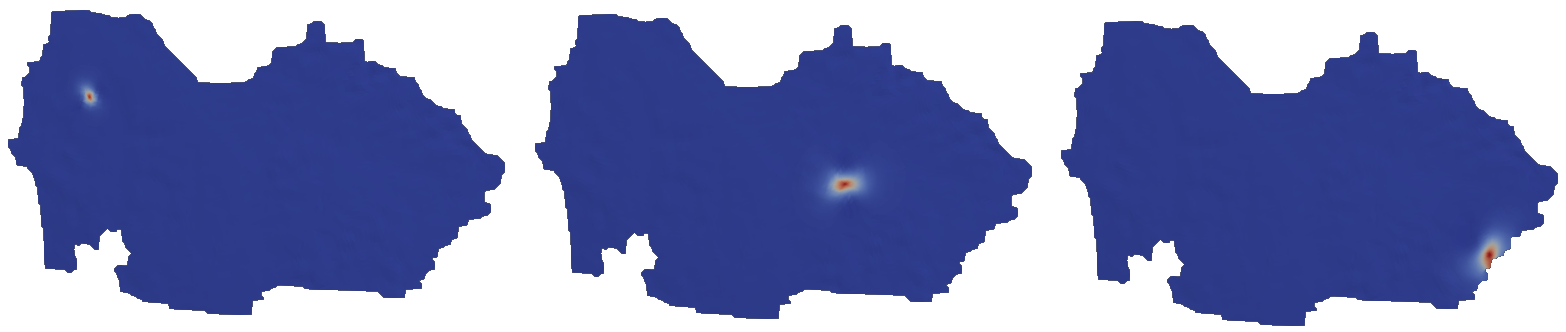
\includegraphics[scale=0.25]{phi_intro.png}
  \end{center}
\end{frame}
% -------------------------------------------------------------------


%\begin{frame}
%	\frametitle{Outline}
%	{\Large
%		\begin{itemize}
%			\setlength\itemsep{2em}
%			\item \textbf{Antartic ice sheet} (background/motivation)
%			{\color{lightgray}\item \textbf{PSF method}}
%			{\color{lightgray}\item \textbf{Numerical results}}	
%		\end{itemize}
%	}
%\end{frame}


\begin{frame}
	\frametitle{Antartic ice sheet}
	
	\vspace{0.2in}
	\begin{columns}
		\begin{column}{0.49\paperwidth}
			\centering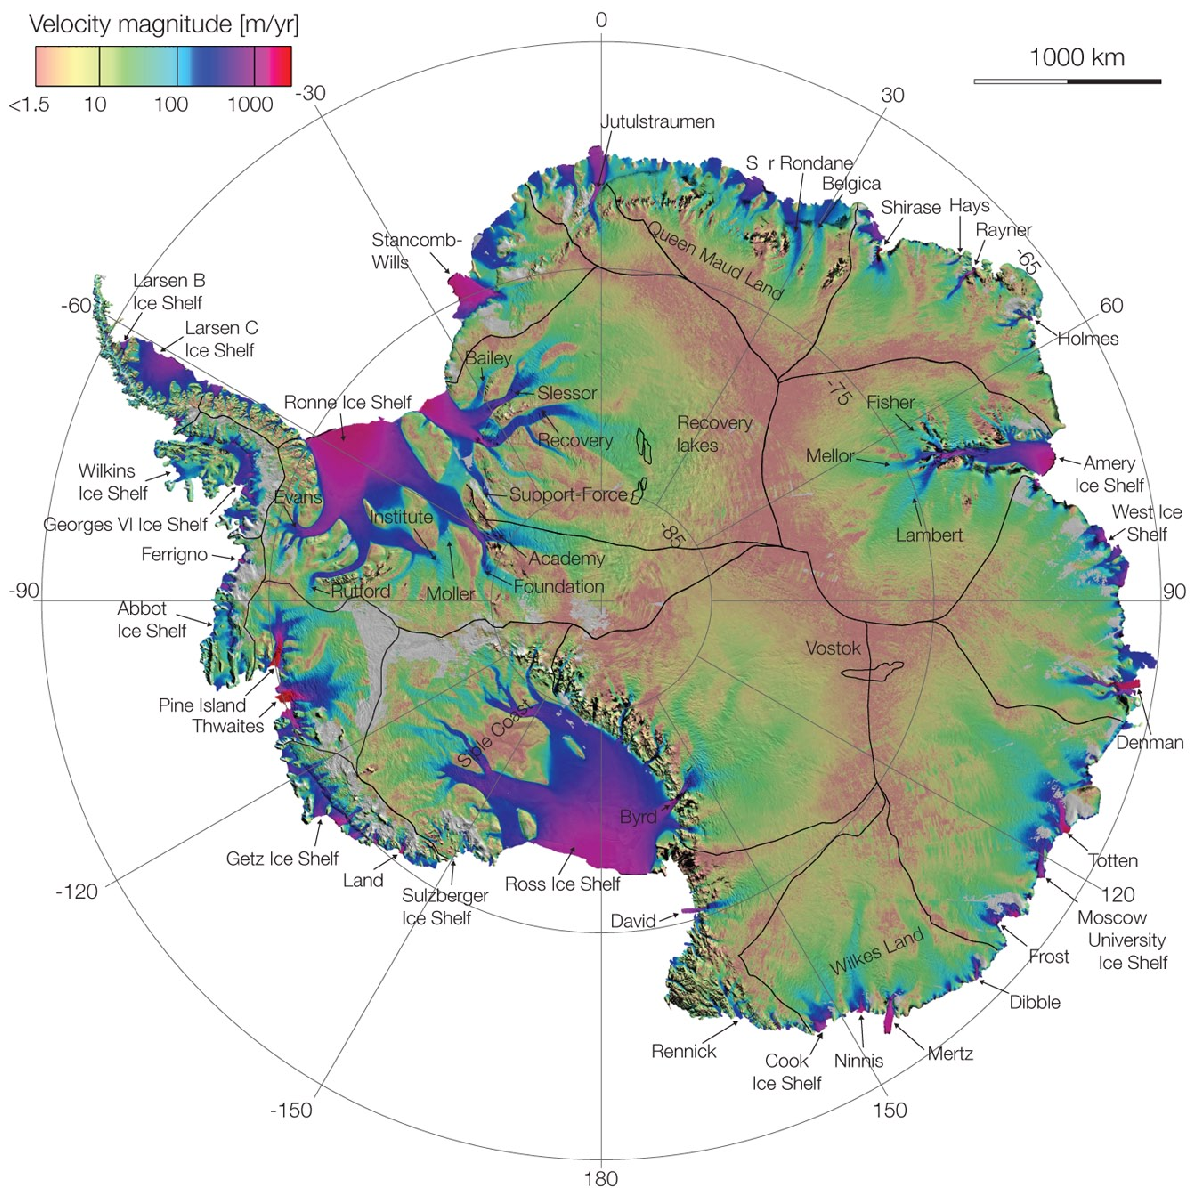
\includegraphics[width=0.7\columnwidth]{ScienceRignot-crop.pdf}
			\vspace{-0.2in}
			\begin{center}
				{\tiny Observed surface flow velocity from InSAR (Rignot et.\ al, 2011)}
			\end{center}
		\end{column}
		\hspace{-0.4in}
		\begin{column}{0.49\paperwidth}
			\vspace{0.1in}
			\centering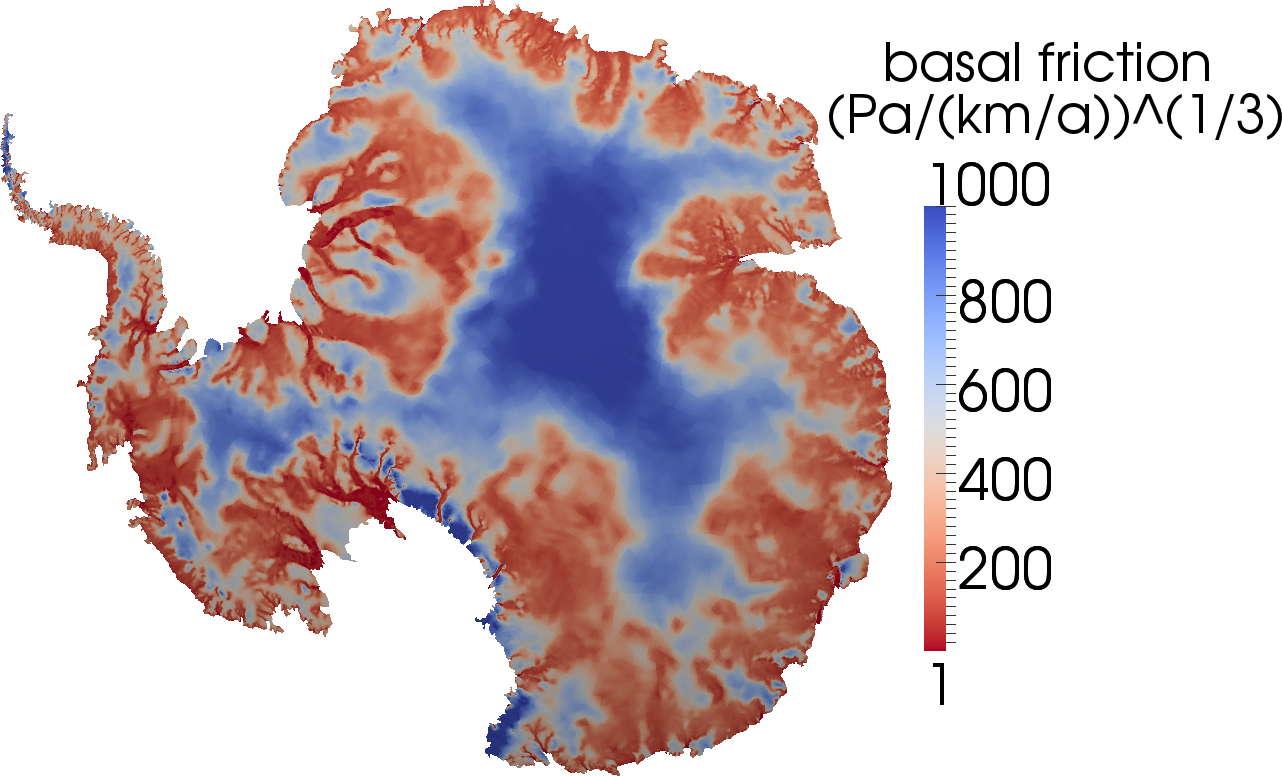
\includegraphics[width=0.85\columnwidth]{beta_cube_cut.png}
			\vspace{-0.1in}
			\begin{center}
				{\tiny Antarctic ice sheet inversion for the basal friction
					parameter field \\
					\vspace{-0.1in}
					from InSAR surface velocities}
			\end{center}
		\end{column}
	\end{columns}
	
	\vspace{0.3in}
	\scriptsize{Details in: T. Isaac, N. Petra, G. Stadler, and
		O. Ghattas. {\em Scalable and efficient algorithms for the
			propagation of uncertainty from data through inference to
			prediction for large-scale problems, with application to flow of
			the Antarctic ice sheet}, Journal of Computational Physics, 296,
		348-368 (2015).}
%	\begin{block}{IPCC Fourth Assessment Report: Climate Change 2007}
%		{\small
%			{\em [T]he uncertainty in the projections of the land ice
%				contributions [to sea level rise] is dominated by the various
%				uncertainties in the land ice models themselves
%				... rather than in the temperature projections.} %[10.A.6]
%		}
%	\end{block}
\end{frame}

%\begin{frame}
%	\frametitle{Outline}
%	{\Large
%		\begin{itemize}
%			\setlength\itemsep{2em}
%			\item \textbf{Ice sheet inverse problem}
%			\item \textbf{Limitations of low rank methods}
%			\item \textbf{New PSF method}
%			\item \textbf{Numerical results}		
%		\end{itemize}
%	}
%\end{frame}

\begin{frame}
	\frametitle{Model problems}
	\begin{figure}
		\centering
		\begin{subfigure}[b]{0.49\textwidth}
			\centering
			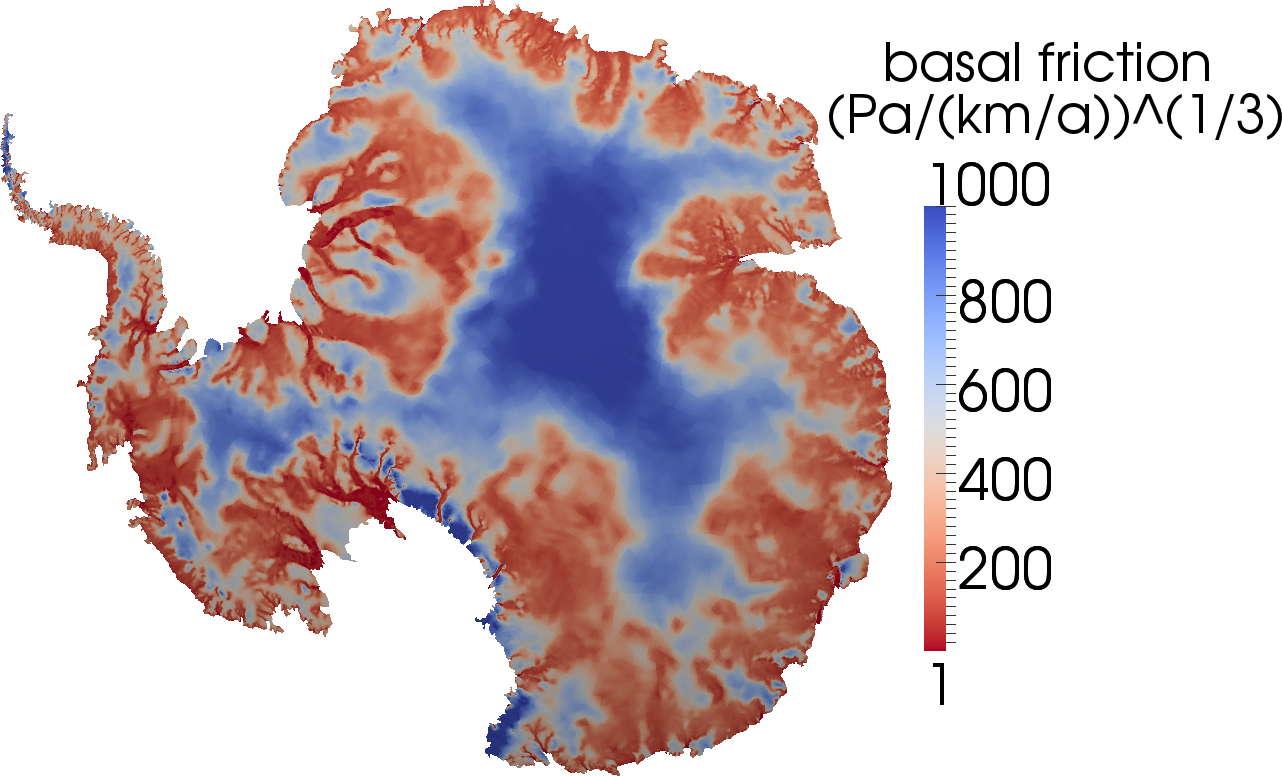
\includegraphics[width=0.9\textwidth]{beta_cube_cut.png}
			\caption{Antartica\\(Ymir)}
		\end{subfigure}
		\hfill
		\begin{subfigure}[b]{0.49\textwidth}
			\centering
			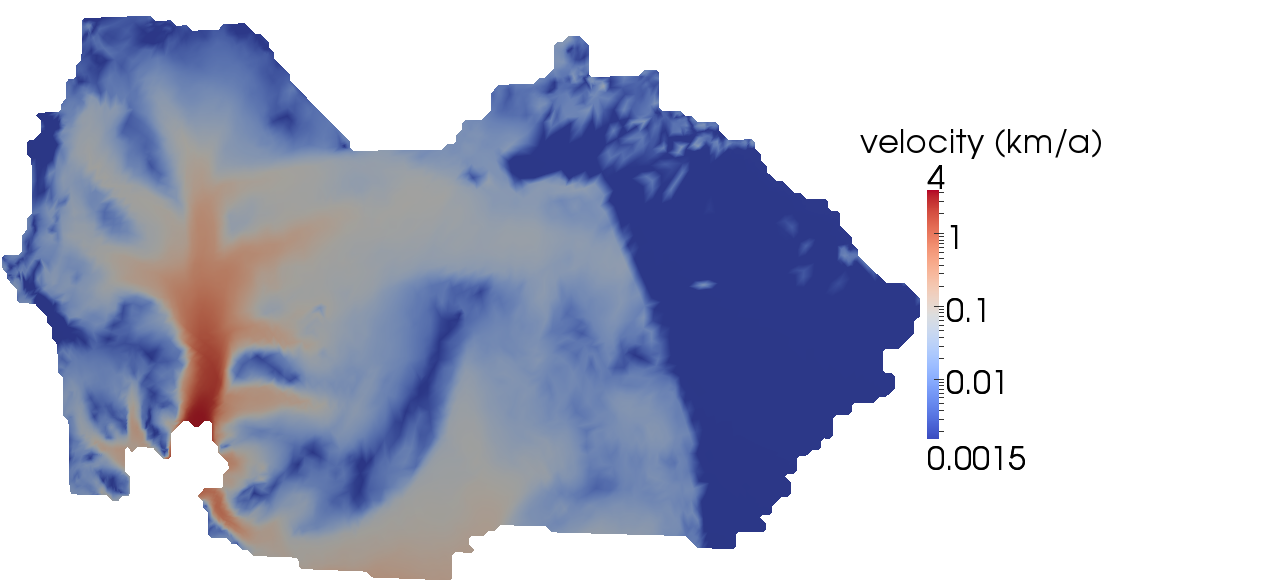
\includegraphics[width=0.9\textwidth]{pig_uobs_uqice.png}
			\caption{Pine Island Glacier\\(Ymir)}
		\end{subfigure}
		\hfill
		\begin{subfigure}[b]{0.49\textwidth}
			\centering
			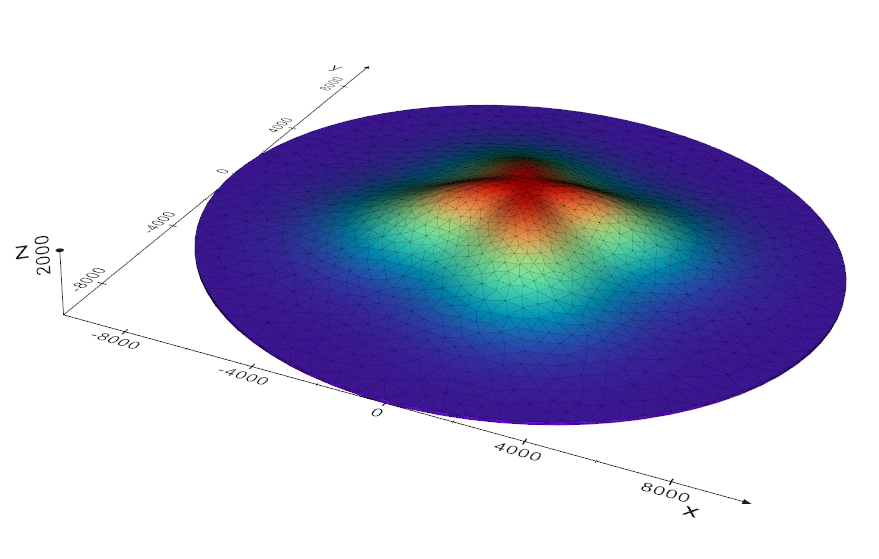
\includegraphics[width=0.9\textwidth]{Mesh_Height.png}
			\caption{Ice Mountain (Hippylib)}
		\end{subfigure}
		\begin{subfigure}[b]{0.49\textwidth}
		\centering
		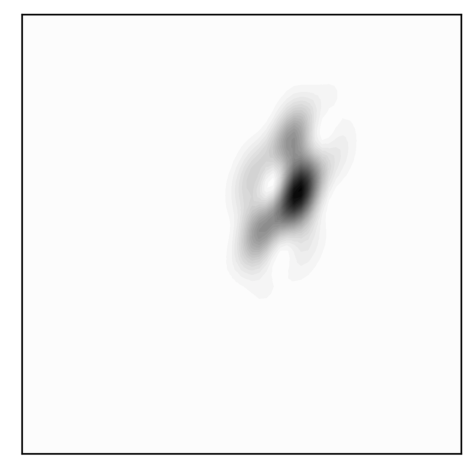
\includegraphics[width=0.7\textwidth]{frog_problem.pdf}
		\caption{Spatially variant blur}
	\end{subfigure}
	\end{figure}
\end{frame}

\begin{frame}
\frametitle{Ice sheet dynamics: forward and inverse}

\begin{block}{Balance of linear momentum, mass, and energy}
  \[
  \begin{aligned}
    % balance of linear momentum:
    - \gbf{\nabla} \cdot \left[ \eta(\theta,\gbf{u}) \, \edot
      -\gbf{I}p \right] &= \rho \gbf{g},
    &[\edot = \tfrac 12  (\gbf{\nabla u} + \gbf{\nabla  u}^T)]
    \hspace{-2em}
    \\
    % balance of mass:
    \gbf{\nabla} \cdot \gbf{u} &= 0,
    \vspace{-2em} \\
    % conservation of energy:
    \rho c \left(\frac{\partial \theta}{\partial t} + \gbf{u} \cdot \gbf{\nabla}
    \theta\right)  - \gbf{\nabla} \cdot (K \gbf{\nabla} \theta)
    &= 2 \, \eta \, \mathrm{tr}(\edot^2)
  \end{aligned}
  \]
\end{block}
\vspace{0.5cm}
\textbf{We have:} Satellite observations of surface velocity

\vspace{0.5cm}

\textbf{We want:} The sliding/friction coefficient $\beta$ in
Robin boundary condition
\begin{equation*}
{\bf T}(\bs \sigma {\bf n}) + \tcr{\beta (x)}{\bf T}{\bf u} = 0
\end{equation*}
($\bf T$ is tangential component)

\end{frame}


%---------------------------------------------------------------------------------%
\begin{frame}
  \frametitle{Bayesian approach} \textbf{Inverse problem:}
  given noisy data $\bs d$ and a model
  $\bs f$, infer parameters $\bs \beta$ that characterize the model, i.e.,
  \begin{equation*}
    \bs f(\bs \beta) + \bs e = \bs d
  \end{equation*}
  Interpret $\bs \beta$, $\bs d$ as random variables;
  solution of inverse problem is the ``posterior'' probability density function
  $\pi_{\mbox{\tiny post}}(\bs \beta)$ found via Bayes' theorem.\\
  \vspace{1em}
  \begin{center}
  	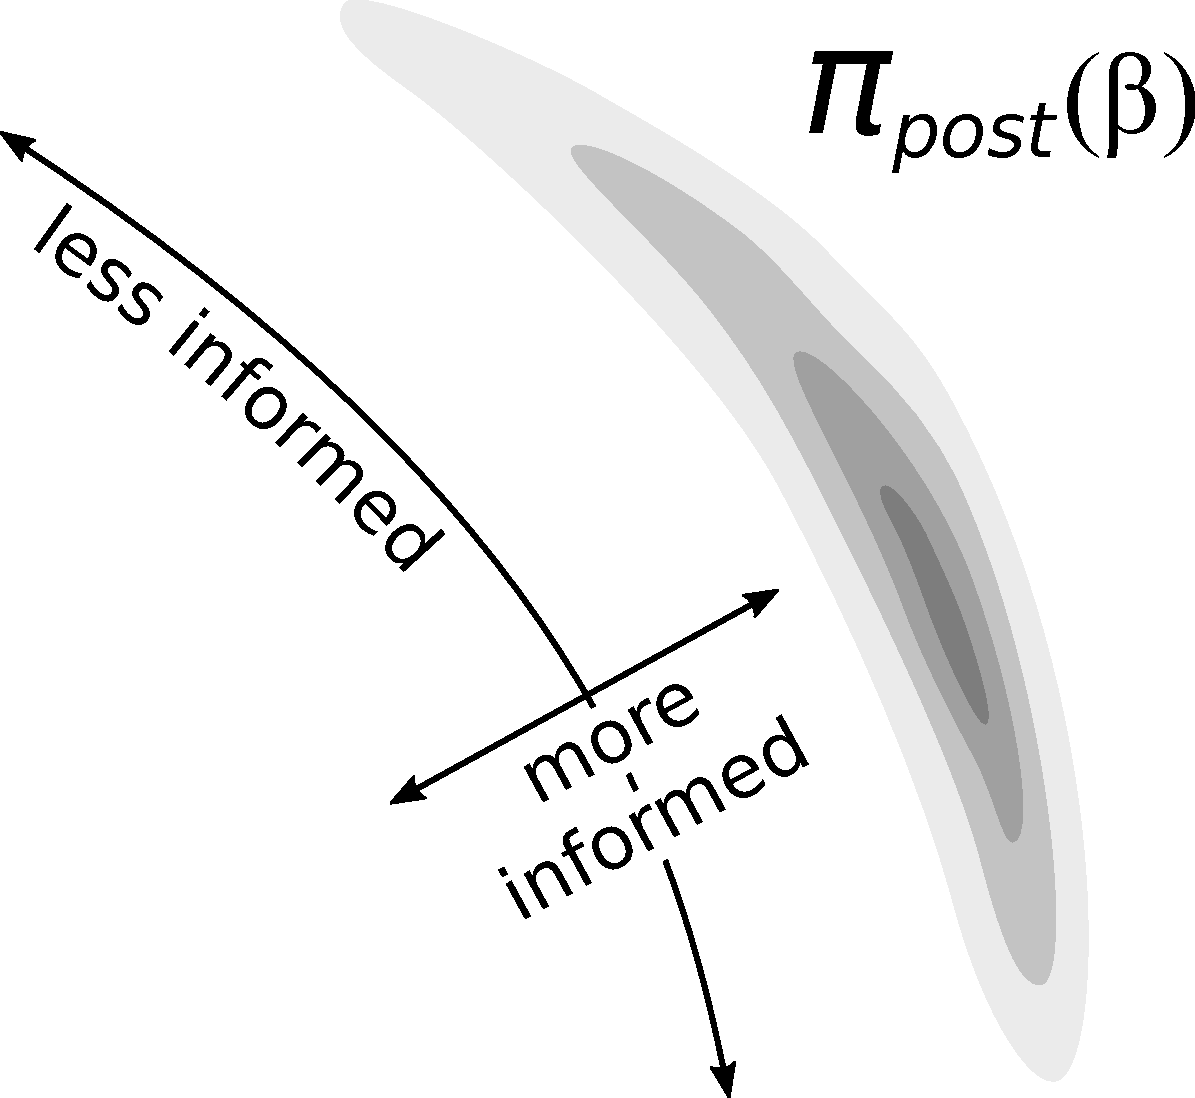
\includegraphics[scale=0.23]{informed_uninformed_modes.pdf}
  \end{center}
\end{frame}

%---------------------------------------------------------------------------------%
%\begin{frame}
%	\frametitle{Ill-conditioning and sampling} 
%	\textbf{Objective:} characterize posterior distribution by drawing samples with Markov chain Monte Carlo.
%	
%	\vspace{0.5cm}
%	\textbf{Dilemma:}
%	If the directional scalings of the proposal distribution are inconsistent with the directional scalings of the posterior, then sampling will be slow.
%	
%	\vspace{0.5cm}
%	\begin{center}
%		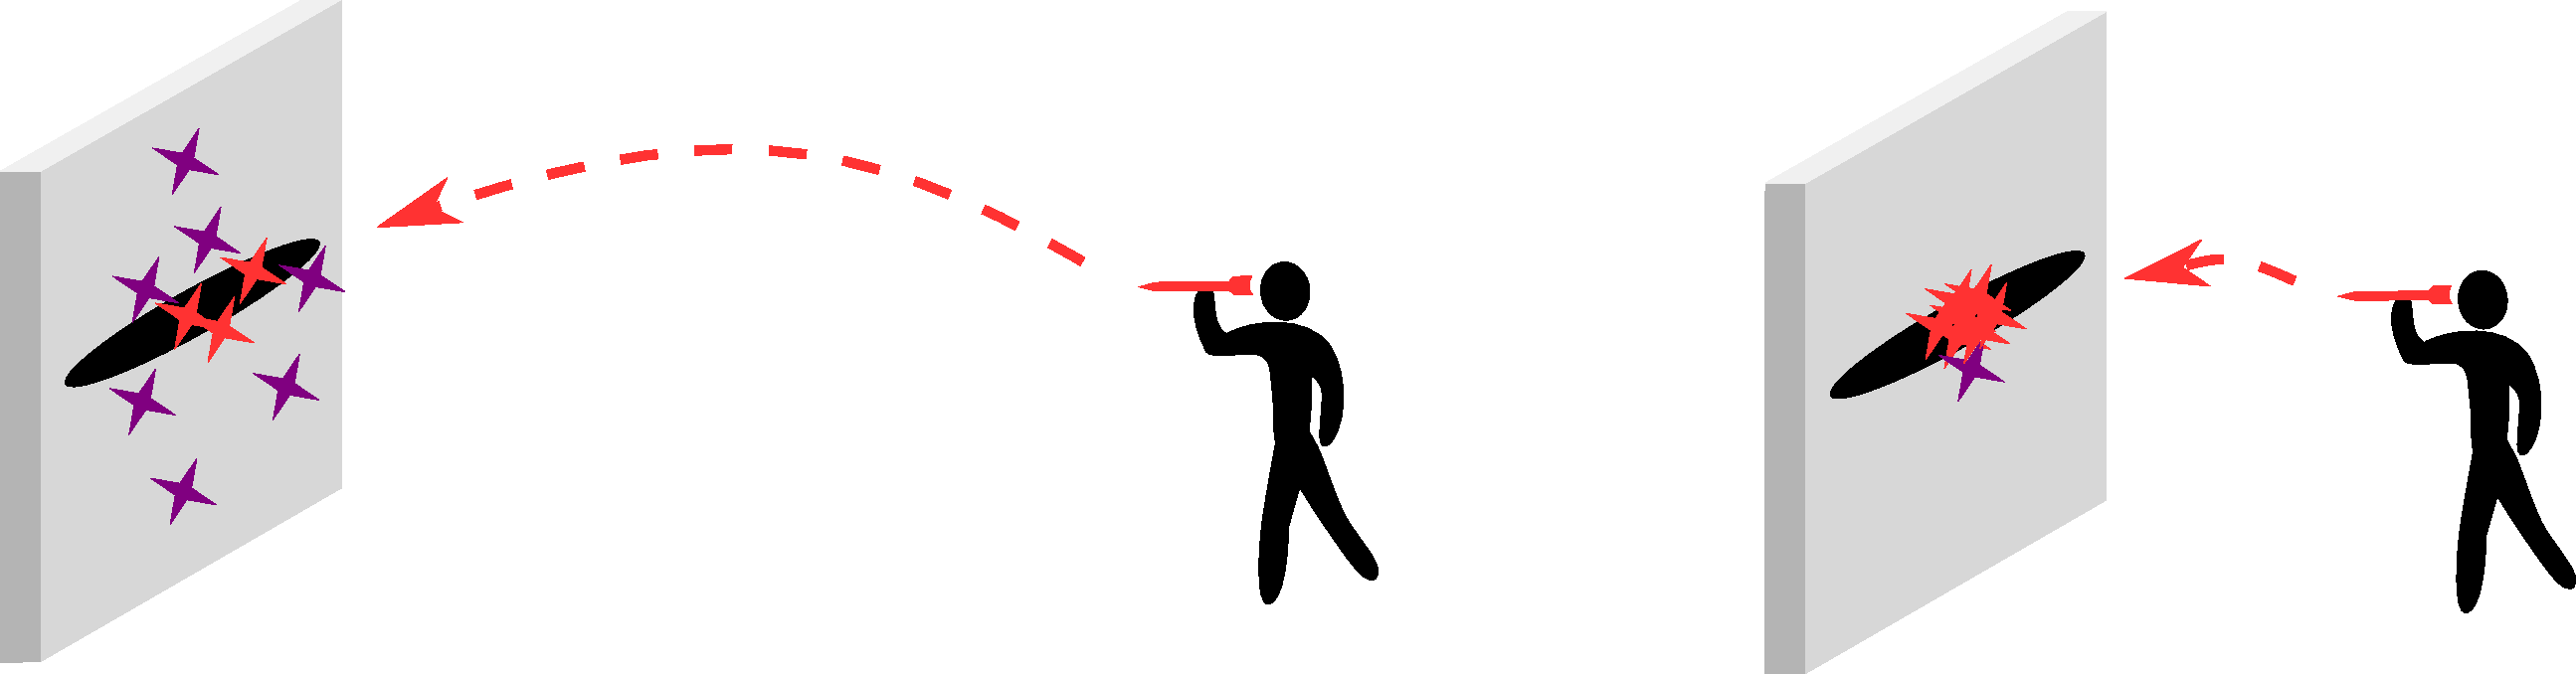
\includegraphics[scale=0.23]{darts_combined.pdf}
%	\end{center}
%\end{frame}


%---------------------------------------------------------------------------------%
\begin{frame}
  \frametitle{Hessian: local Gaussian approximation}
  
  \newcommand{\proposal}{\bs y}
  \newcommand{\params}{\bs m}
  
  \textbf{Local Gaussian approximation proposal:}
  \begin{align*}
  \pi_\text{prop}(\beta) := \frac { \det \bs H^{1/2} }{(2\pi)^{n/2} }
  \exp \left( - \frac 12 \left( \proposal - \bs{\beta}_k + \bs H^{-1} \bs
  g \right) ^T \bs H \left( \proposal - \bs{\beta}_k + \bs H^{-1} \bs g \right)
  \right)
  \end{align*}
  
  \vspace{0.25cm}

  \begin{center}
  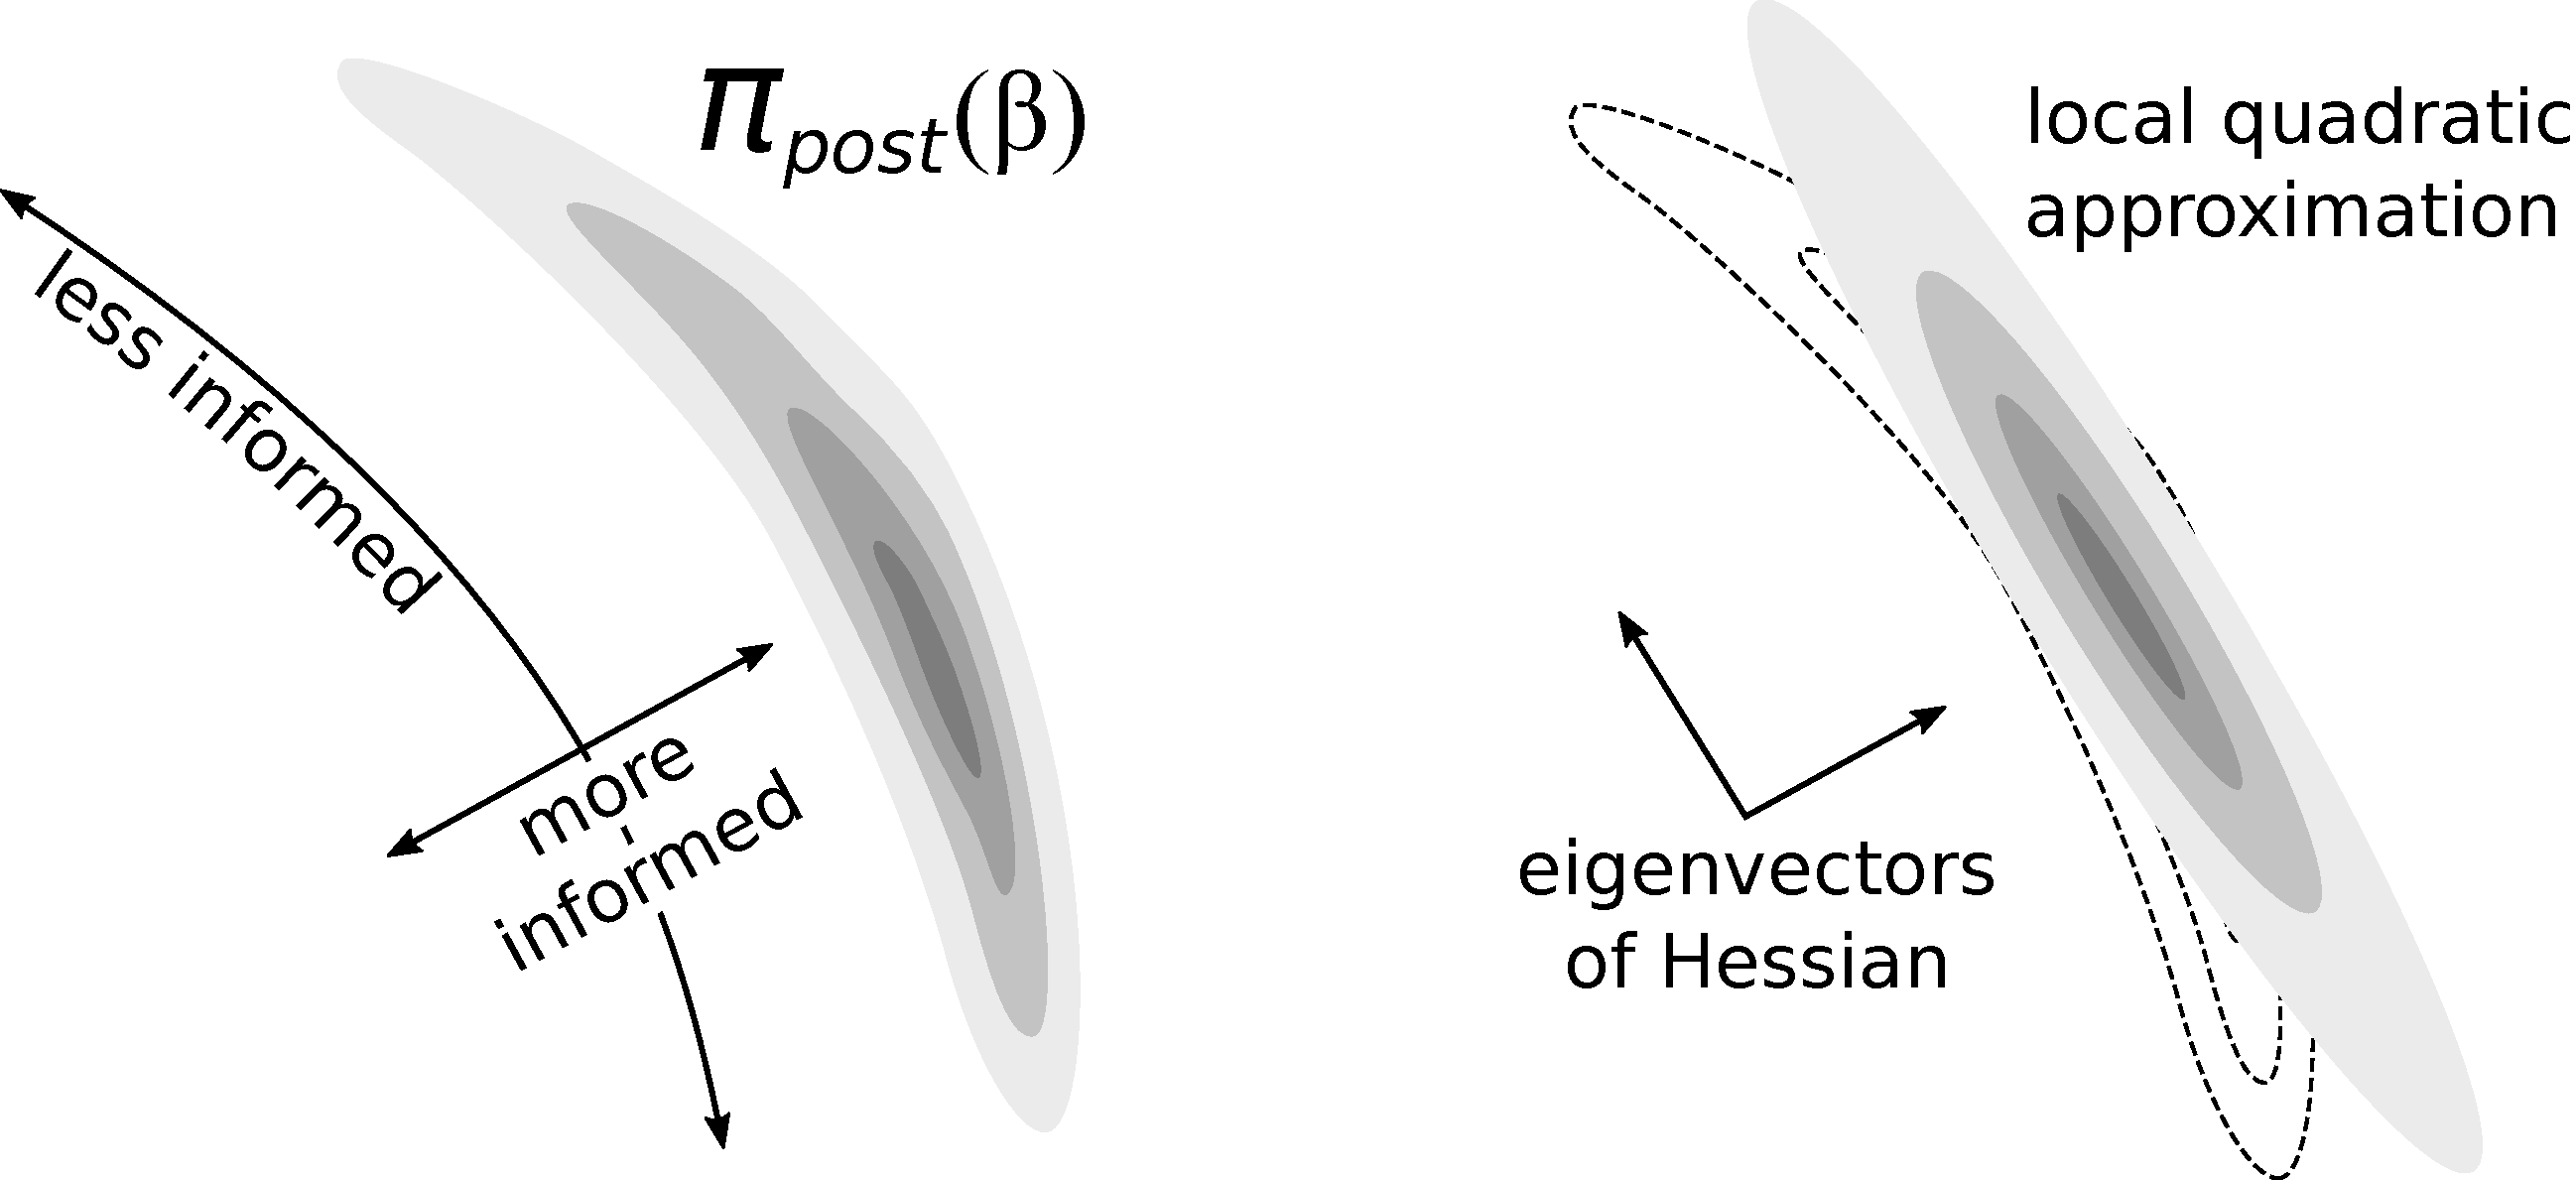
\includegraphics[scale=0.25]{informed_uninformed_modes_combined.pdf}
  \end{center}
\end{frame}
%---------------------------------------------------------------------------------%
\begin{frame}
	\frametitle{Matrix-free}
	
	$$\mathbf{H} = \underbrace{\mathbf{H}_d}_{\text{data misfit Hessian}} + \underbrace{\mathbf{H}_r}_\text{Prior Hessian}$$
	
	\begin{itemize}
		\setlength\itemsep{2em}
		\item Data misfit Hessian, and therefore the whole Hessian, are only available matrix-free
		\item Cannot access $\mathbf{H}_{ij}$ easily
		\item Can compute matrix-vector products (matvecs)
		$$\mathbf{u} \mapsto \mathbf{H} \mathbf{u}$$
		\item Cost: \textbf{2} linearized Stokes \textbf{PDE solves} per matvec
	\end{itemize}
	
\end{frame}

\begin{frame}
	\frametitle{Low rank Hessian approximation (extremely expensive!)}
	
	\textbf{Low-rank approximation/Woodbury formula}:
	
	\[
	\Hmatrix^{-1} =
	\left ( {\bs{H}_d} + \mathbf{H}_r \right)^{-1}
	\approx \mathbf{H}_r^{1/2} (\bs{V}_r \bs{\Lambda}_r \bs{V}^T_r + \bs{I})^{-1}
	\mathbf{H}_r^{1/2} 
	% - \bs{V}_r \bs{D}_r \bs{V}^T_r
	\]
	where $\bs{V}_r$ and $\bs{\Lambda}_r$ are the eigenvectors/values of
	%  the eigenvalue problem 
	$\bs{H}_d \bs{v}_i = \lambda_i \mathbf{H}_r \bs{v}_i $
	\begin{center}
		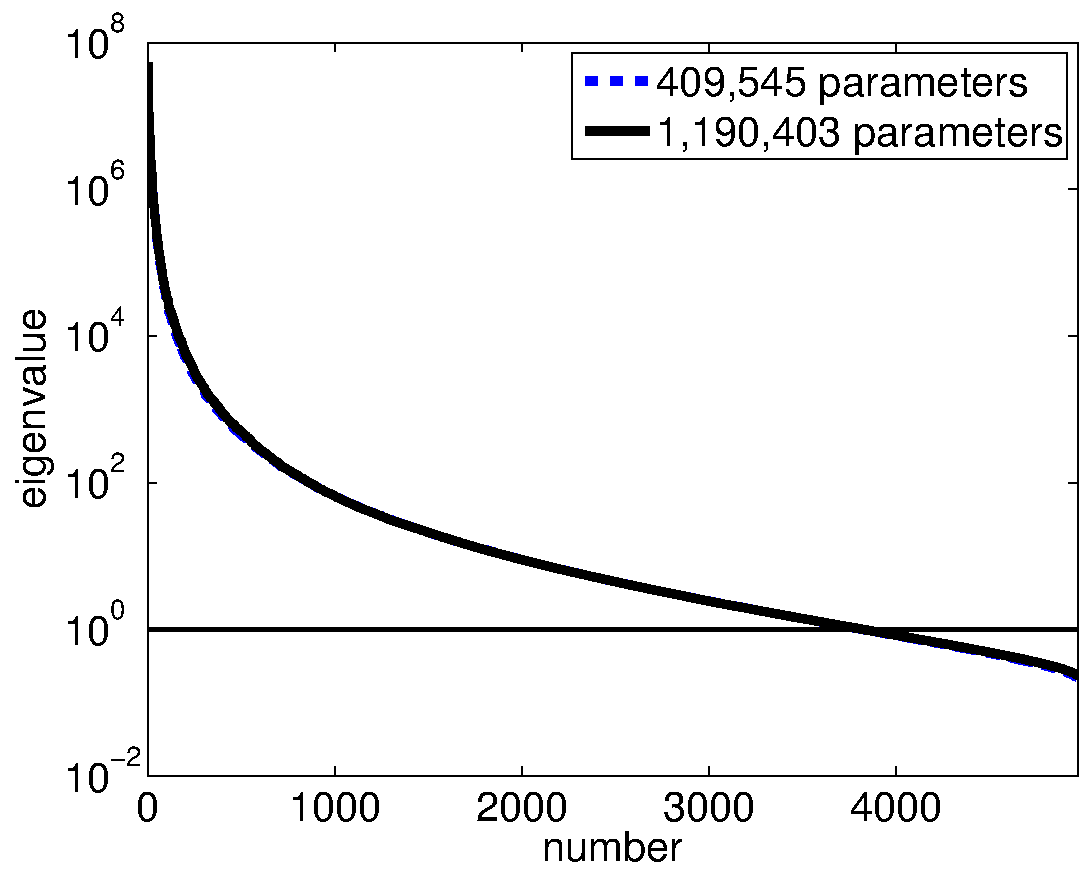
\includegraphics[width=0.5\textwidth]{spec_ppmisfit_hess_coarseandfine_new.pdf}
	\end{center}
	
	\begin{itemize}
		\item [] \scriptsize{Details in: T. Isaac, N. Petra, G. Stadler, and
			O. Ghattas. {\em Scalable and efficient algorithms for the
				propagation of uncertainty from data through inference to
				prediction for large-scale problems, with application to flow of
				the Antarctic ice sheet}, Journal of Computational Physics, 296,
			348-368 (2015).}
	\end{itemize}
\end{frame}
%---------------------------------------------------------------------------------%
%\begin{frame}
%	\frametitle{MCMC sampling: stochastic Newton}
%	\framesubtitle{Performance results / Convergence diagnostics}
%	%\vspace{0.1in}
%	\small
%	
%	\newcommand{\proposal}{\bs y}
%	\newcommand{\params}{\bs m}
%	
%	
%	\only<1>{
%		\begin{table}[t]
%			\begin{center}
%				%\def\firstrowcolor{}
%				%\def\secondrowcolor{}
%				%\only<1>{\def\firstrowcolor{\rowcolor{gray}}}
%				%\only<2>{\def\secondrowcolor{\rowcolor{red}}}
%				\begin{tabular}{|l|c|c|c|c|c|c|c|}
%					\hline\hline
%					{} & {\bfseries MPSRF} & {\bfseries IAT} & {\bfseries ESS} & {\bfseries
%						MSJ} & {\bfseries ARR} & {\bfseries $\#$Stokes} & {\bfseries time (s)}\\
%					\hline%\hline
%					%\multicolumn{8}{|c|}{small noise case (more Gaussian) }\\
%					%\hline
%					%ind. sampler & 1.210 & 253 & 2075  & 1456 & 41 & 2783  & 139\\
%					%frozen Hessian  & 1.001 & 6 & 84004 & 1390 & 40 & 72     & 4  \\
%					%dynamic Hessian & 1.073 & 125 & 4032  & 565  & 17 & 1375 & 69\\
%					%\hline
%					%\multicolumn{8}{|c|}{large noise case (more non-Gaussian)}\\
%					%\hline
%					%SNIS  & 1.507 & 435 & 1207 & 280 & 9  & 4350 &  218\\
%					%SNMAP  & 1.045 & 80 & 6563 & 190  & 6  & 960  & 48 \\
%					SN & 1.348 & 600 & 875  & 64   & 2  & {\bf \alert{8400}} & 420 \\
%					\hline\hline
%				\end{tabular}
%			\end{center}
%		\end{table}
%	}
%	\vspace{-0.05in}
%	
%	\begin{columns}
%		\begin{column}{0.45\columnwidth}
%			\begin{itemize}
%				\item {\bfseries MPSRF:} multivariate potential scale reduction factor
%				\vspace{-0.02in}
%				\item {\bfseries IAT:} integrated autocorrelation time
%				\vspace{-0.02in}
%				\item {\bfseries ESS:} effecitive sample size
%				\vspace{-0.02in}
%				\item {\bfseries MSJ:} mean squared jump distance
%			\end{itemize}
%		\end{column}
%		\begin{column}{0.45\columnwidth}
%			\begin{itemize}
%				\item {\bfseries ARR:} average rejection rate
%				\vspace{-0.02in}
%				\item {\bfseries $\#$Stokes:} $\#$ of Stokes solves per independent sample
%				\vspace{-0.02in}
%				\item {\bfseries time:} time per independent sample
%			\end{itemize}
%		\end{column}
%	\end{columns}
%	
%	\begin{columns}
%		\hspace{0.26in}
%		\begin{column}{0.95\columnwidth}
%			\begin{itemize}
%				\item {\bfseries Statistics:} 21 parallel chains (each 25k); $\#$
%				samples: 525k; dof: 139; rank Hessian: 15
%				%\item SNIS, SNMAP and SN are variants of the stochastic Newton
%				%  MCMC method
%			\end{itemize}
%		\end{column}
%		\begin{column}{0.5\columnwidth}
%		\end{column}
%	\end{columns}
%	
%	\vspace{0.05in}
%	
%	\begin{center}
%	{\huge Too many PDE solves!!}
%	\end{center}
%	\vspace{0.05in}
%	
%	\begin{itemize}
%		\item [] \scriptsize{Details in: N. Petra, J. Martin, G. Stadler,
%			O. Ghattas. {\em A computational framework for
%				infinite-dimensional Bayesian inverse problems: Part
%				II. Stochastic Newton MCMC with application to ice sheet inverse
%				problems}, SIAM Journal on Scientific Computing, 2014}
%	\end{itemize}
%	
%\end{frame}
%---------------------------------------------------------------------------------%

%---------------------------------------------------------------------------------%
%\begin{frame}
%	\frametitle{Outline}
%	{\Large
%		\begin{itemize}
%			\setlength\itemsep{2em}
%			{\color{lightgray}\item \textbf{Antartic ice sheet} (background/motivation)}
%			\item \textbf{PSF method}
%			{\color{lightgray}\item \textbf{Numerical results}}	
%		\end{itemize}
%	}
%\end{frame}
%---------------------------------------------------------------------------------%
%---------------------------------------------------------------------------------%
%Story:
%
%Existing Hessian approximations are based on low-rank approximation
%methods, which require computing twice as many linearized forward or
%adjoint partial differential equation (PDE) solves as the numerical
%rank of the Hessian.
%
%These methods are inefficient when the numerical rank of the Hessian
%is large, as is the case in continental scale ice sheet inverse
%problems.
%
%Our goal is to take advantage of the off-diagonal low-rank structure
%of the Hessian and use {\note hierarchical matrix compression} to
%reduce the computational cost of solving the Bayesian ice sheet
%inverse problem.
%---------------------------------------------------------------------------------%
\begin{frame}
	\frametitle{Hierarchical matrices ($\mathcal{H}$-matrices)}
	\begin{itemize}
		\item Matrix is reordered and subdivided recursively
		\item Many off-diagonal blocks are low-rank
		\item Overall matrix may be high rank
		\item $O(N \left(\log N\right)^a)$ complexity matrix operations, $a \in \{0,1,2,3\}$
		\begin{itemize}
			\item matrix-vector products, matrix-matrix addition, matrix-matrix multiplication, matrix factorization, matrix inversion, ...
		\end{itemize}
	\end{itemize}
	\begin{center}
		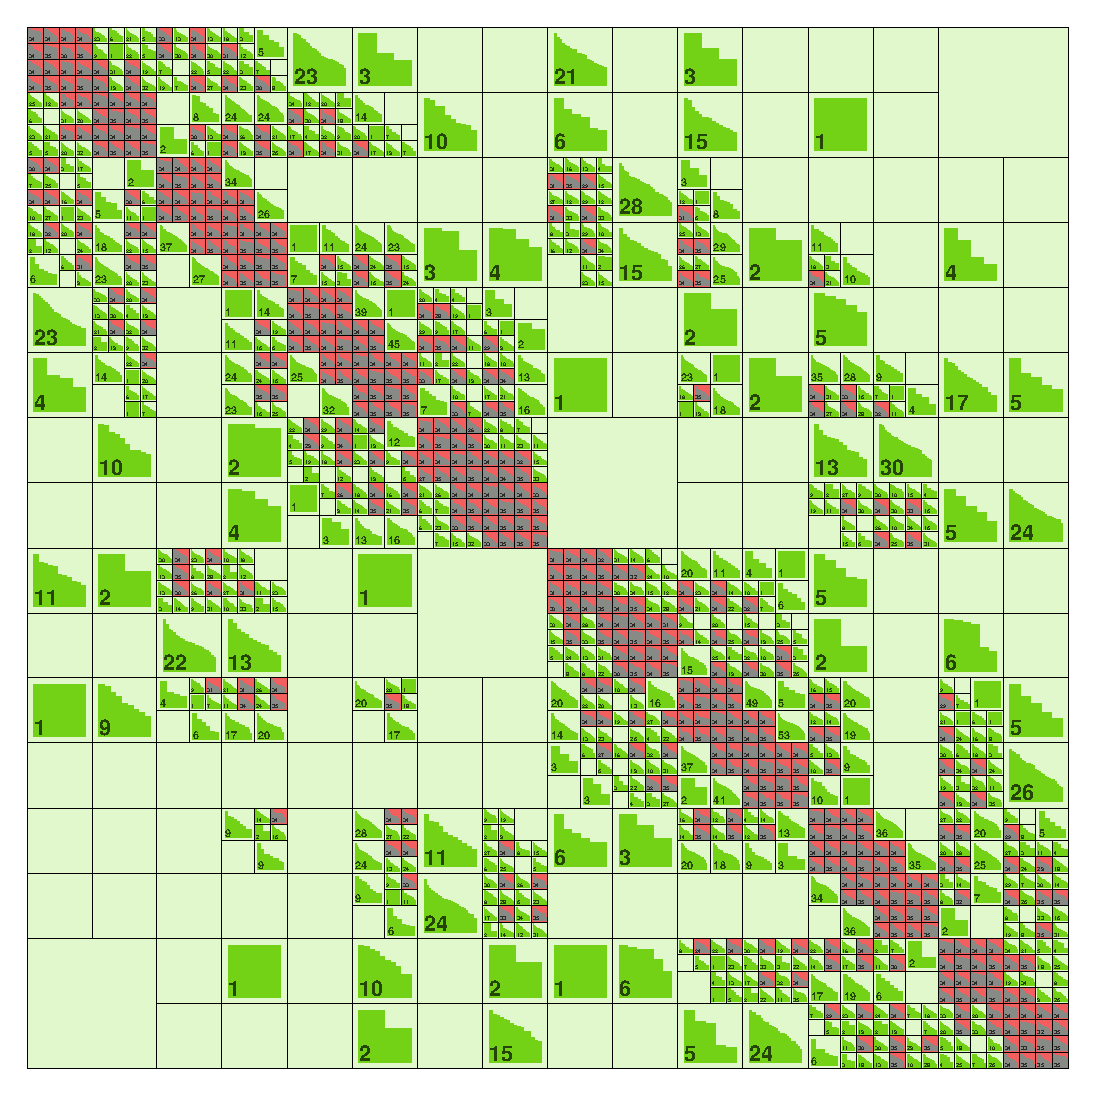
\includegraphics[width=0.45\textwidth]{heat_inverse_problem_Hfull_hmatrix.eps}
	\end{center}
\end{frame}

\begin{frame}
	\frametitle{Hierarchical matrix vs. matrix free}
	\begin{itemize}
		\setlength\itemsep{1.5em}
		\item Classical methods for building $\mathcal{H}$-matrix require matrix entries $\mathbf{H}_{ij}$ 
		\item New algebraic methods based on ``peeling process'' can build $\mathcal{H}$-matrix from matrix-vector products
		\begin{itemize}
			\item {\scriptsize Ambartsumyan, Boukaram, Bui-Thanh, Ghattas, Keyes, Stadler,
				Turkiyyah, and Zampini, "Hierarchical matrix approximations of Hessians arising in inverse problems governed by PDEs", SISC, 2020.}
			\item {\scriptsize Hartland, Tucker Andrew, et al. "Hierarchical off-diagonal low-rank approximation of Hessians in inverse problems, with application to ice sheet model initialization." Inverse Problems (2023).}
		\end{itemize} 
		\item \textbf{Problem:} peeling process better than low rank, but \textbf{still expensive}
		\item Here we build the $\mathcal{H}$-matrix faster by taking advantage of the problem structure
		\begin{itemize}
			\item \textbf{Local sensitivities}
			\item \textbf{Local mean-displacement invariance}
			\item \textbf{Non-negative impulse responses*}
		\end{itemize}
	\end{itemize}
\end{frame}

\begin{frame}
	\frametitle{Local sensitivities}
	\center
	 \begin{tikzpicture}
	\fill[red!90,nearly transparent] (5,0) -- (7,.5) -- (3,.5) -- (1,0) -- cycle;
	\draw [fill=red!40!white,opacity=1] (3,2.25) -- (3.5,2.25) -- (3.25,.25) -- cycle;
	\draw [fill=red] (3.25,2.25) circle (.25cm and 0.07cm);
	\draw (3.25,2.25) -- (2,3);
	\draw [thick] (2,3) node[above]{sensitivities, $\frac{\partial u}{\partial\beta_j}$};
	\draw[red,dashed] (7,.5) -- (3,.5) -- (1,0);
	\draw [fill=blue!40!white,opacity=1] (4.25,.25) -- (4.5,2.25) -- (4.75,.25) -- cycle;
	\draw [fill=blue] (4.5,.25) circle (.25cm and 0.07cm);
	\draw (4.5,.25) -- (2,-.5);
	\draw [thick] (2,-.5) node[below]{sensitivities, $\frac{\partial u_i}{\partial\beta}$};
	\draw (1,0) -- (5,0) -- (5,2) -- (1,2) -- (1,0);
	\draw  (5,2) -- (7,2.5) -- (3,2.5) -- (1,2);
	\draw  (7,2.5) -- (7,.5) -- (5,0);
	\draw  (5,2.25) -- (6,3) ;
	\draw [thick] (6,3) node[above]{measurements, $\boldsymbol{d}$};
	\draw[red]   (5.5,.25) -- (5.5,.125) ;
	\draw  (5.5,.125) -- (5.5,-.5) ;
	\draw [thick] (5.5,-.5) node[below]{parameter, $\beta(x)$};
	
	\draw[dashed] (3,.5) -- (3,2);
	\draw[blue,dashed] (3,2) -- (3,2.5);
	\fill[blue!90,nearly transparent] (5,2) -- (7,2.5) -- (3,2.5) -- (1,2) -- cycle;
	\end{tikzpicture}
\end{frame}
%---------------------------------------------------------------------------------%
\begin{frame}
	\frametitle{Local mean-displacement invariance}
	\begin{center}
		\textbf{Impulse response $\phi_x$:}
		\begin{align*}
		\phi_x := H_d~ \delta_x =& \text{ action of Hessian operator on delta distribution at x} \\
		\mu(x) :=& \text{ center of mass (mean) of }\phi_x
		\end{align*}
		
		\vspace{1em}
		
		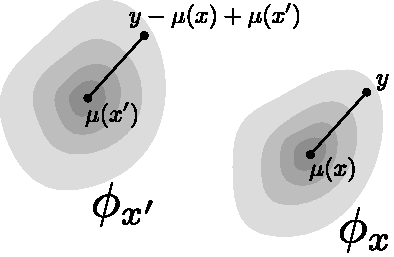
\includegraphics[width=0.5\columnwidth]{mean_displacement_invariance.pdf}
		
		\vspace{1em}
		
		\textbf{Local mean-displacement invariance:}
		$$\phi_x(y) \approx \phi_{x'}(y-\mu(x) + \mu(x'))$$
		
		%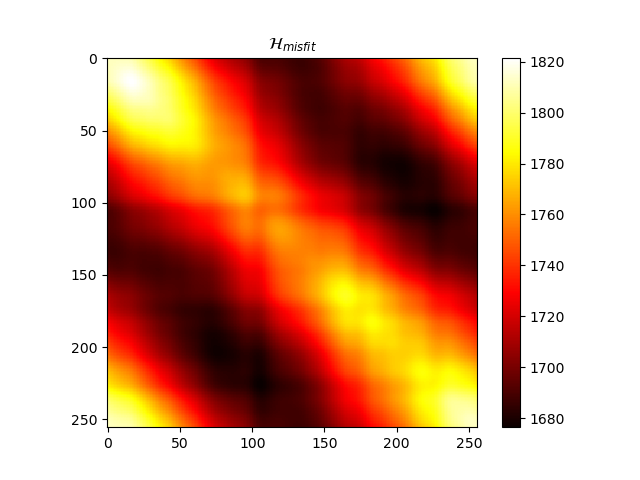
\includegraphics[width=0.6\columnwidth]{Hess1_ordered.png}
	\end{center}
\end{frame}

\begin{frame}
	\frametitle{Impulse responses are ``columns'' of the integral kernel}
	\begin{center}

	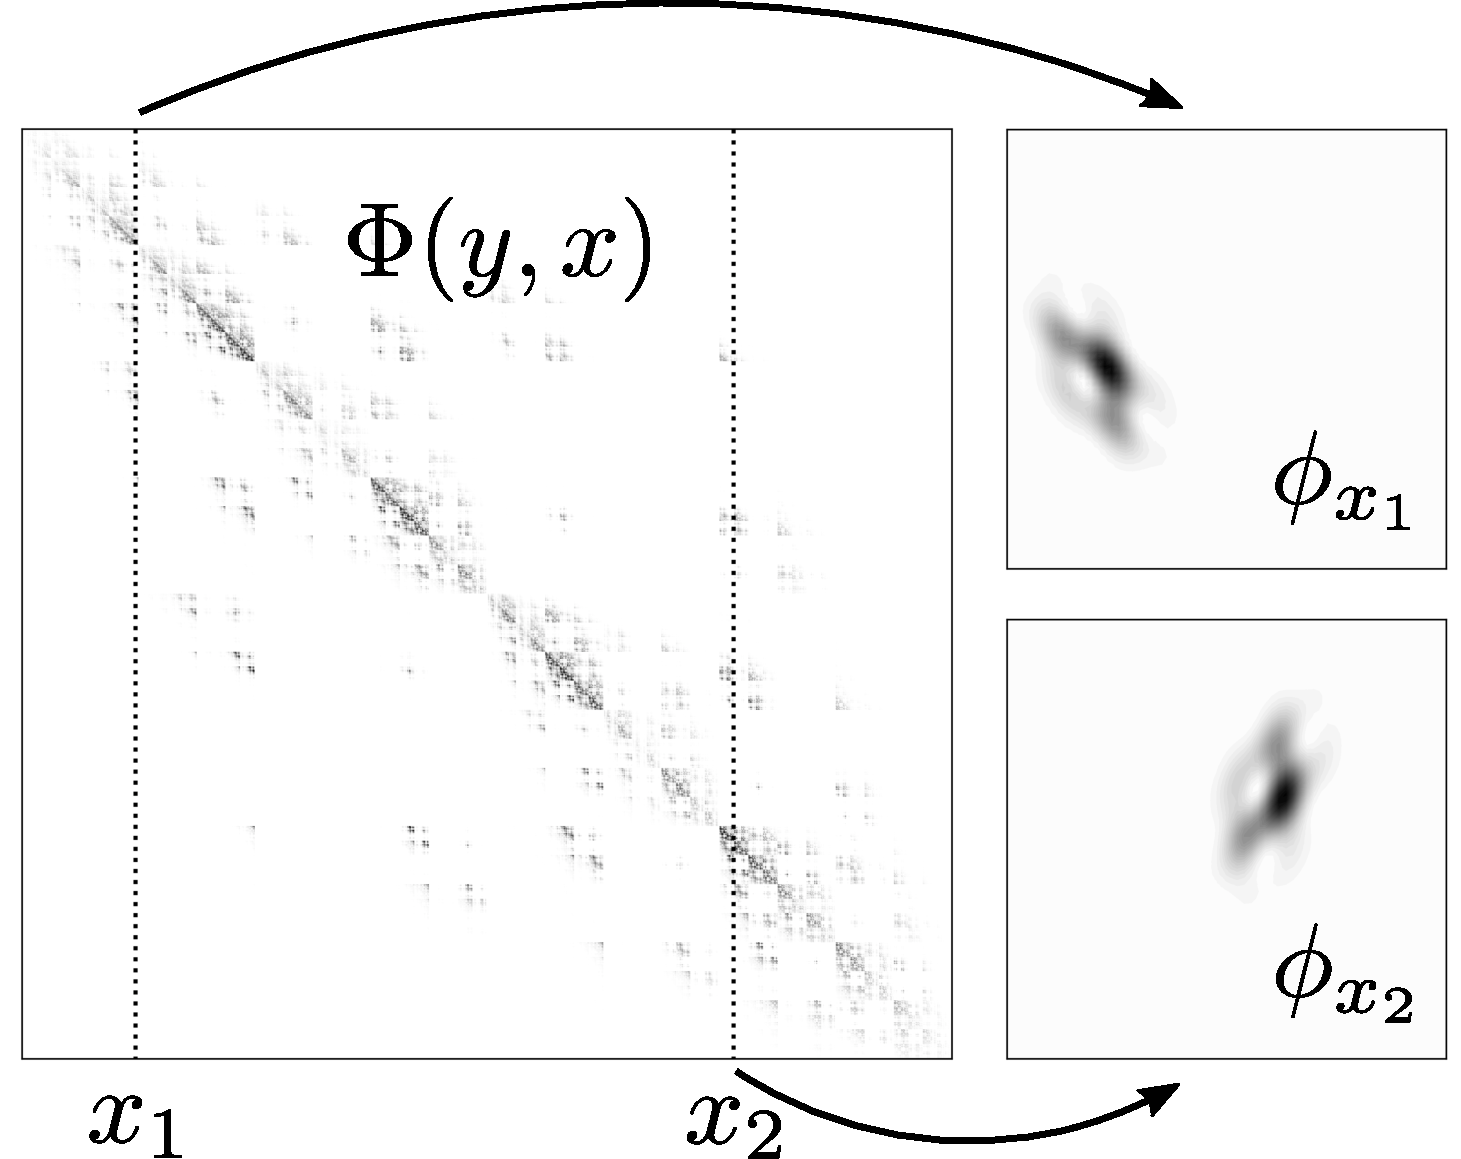
\includegraphics[width=0.7\columnwidth]{kernel_impulse_illustration2.pdf}
		
	\end{center}
\end{frame}
%---------------------------------------------------------------------------------%
\begin{frame}
 \frametitle{Hessian impulse responses (Pine Island Glacier)}
 \center
	\only<1>{
		\begin{center}
			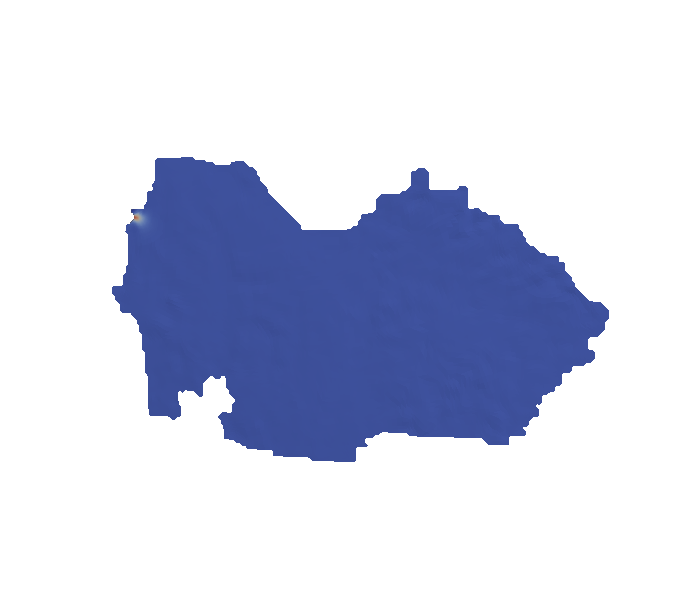
\includegraphics[width=1.0\columnwidth]{reordered_phi/phi0_minimal.png}
		\end{center}
	}
	\only<2>{
	\begin{center}
		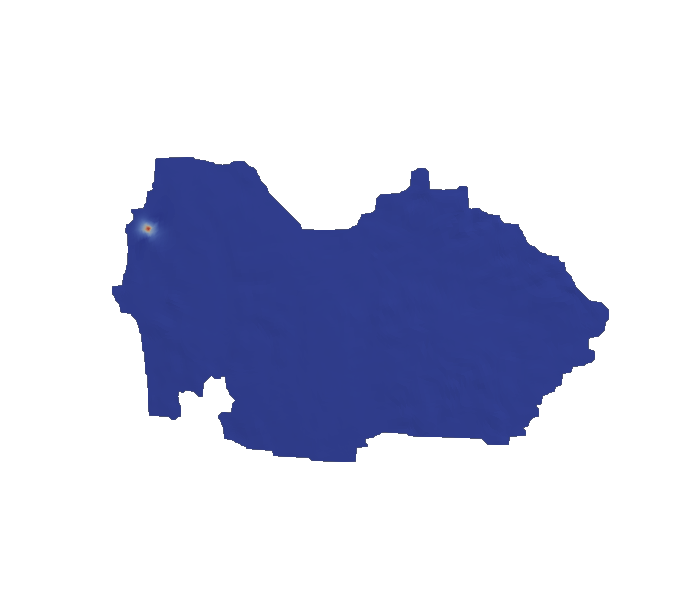
\includegraphics[width=1.0\columnwidth]{reordered_phi/phi1_minimal.png}
	\end{center}
	}
	\only<3>{
	\begin{center}
		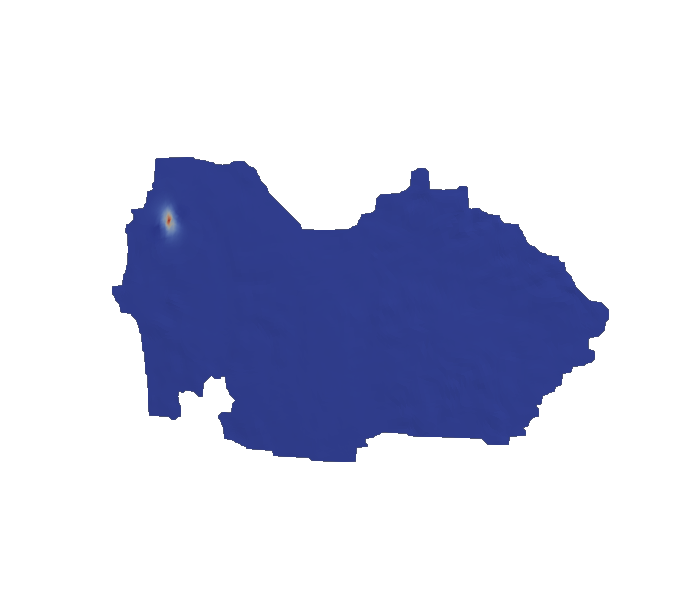
\includegraphics[width=1.0\columnwidth]{reordered_phi/phi2_minimal.png}
	\end{center}
}
	\only<4>{
	\begin{center}
		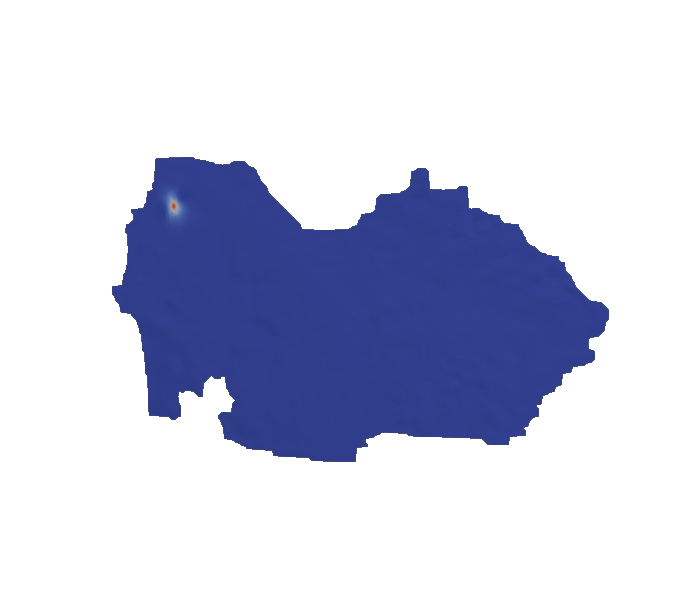
\includegraphics[width=1.0\columnwidth]{reordered_phi/phi3_minimal.png}
	\end{center}
}
	\only<5>{
	\begin{center}
		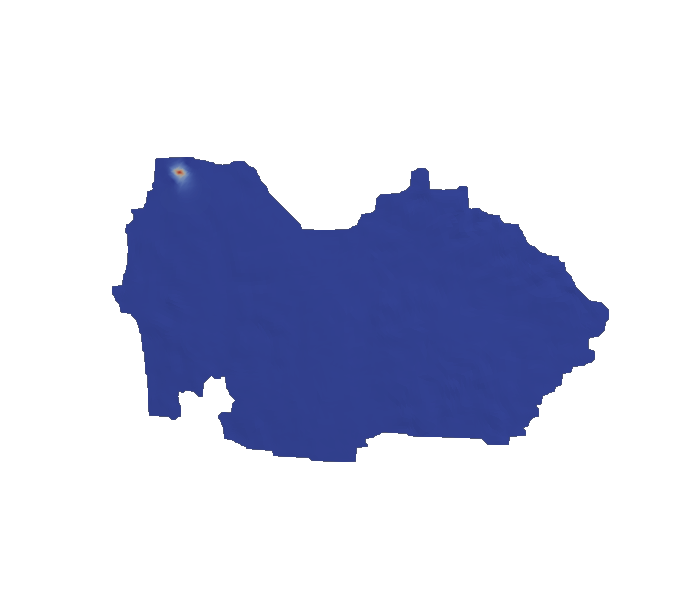
\includegraphics[width=1.0\columnwidth]{reordered_phi/phi4_minimal.png}
	\end{center}
}
	\only<6>{
	\begin{center}
		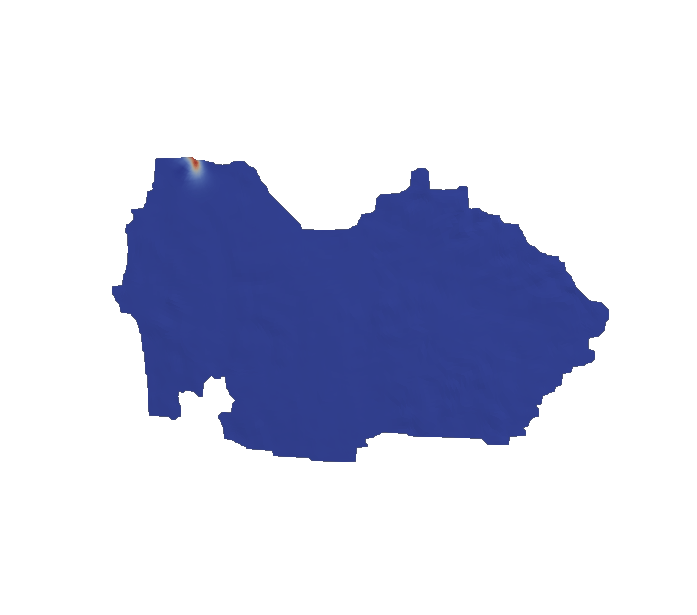
\includegraphics[width=1.0\columnwidth]{reordered_phi/phi5_minimal.png}
	\end{center}
}
	\only<7>{
	\begin{center}
		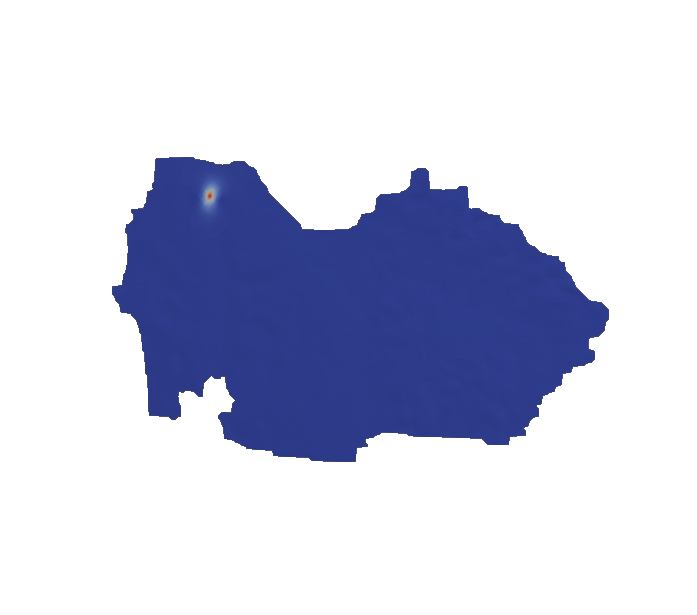
\includegraphics[width=1.0\columnwidth]{reordered_phi/phi6_minimal.png}
	\end{center}
}
	\only<8>{
	\begin{center}
		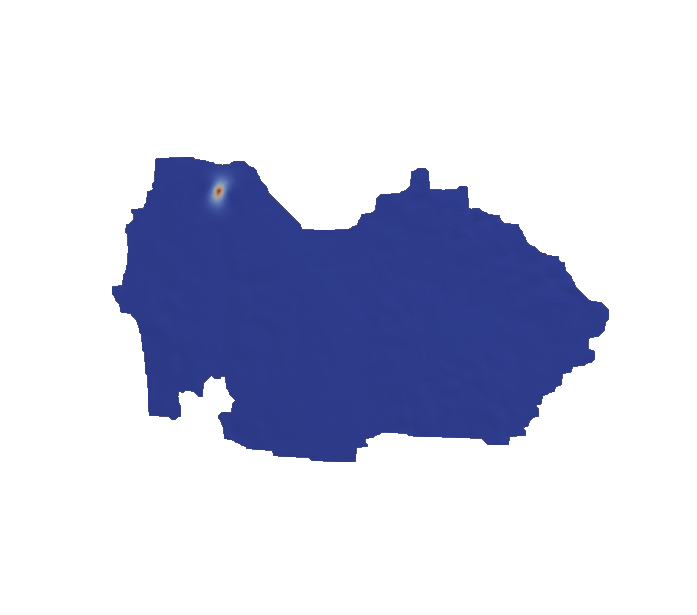
\includegraphics[width=1.0\columnwidth]{reordered_phi/phi7_minimal.png}
	\end{center}
}
	\only<9>{
	\begin{center}
		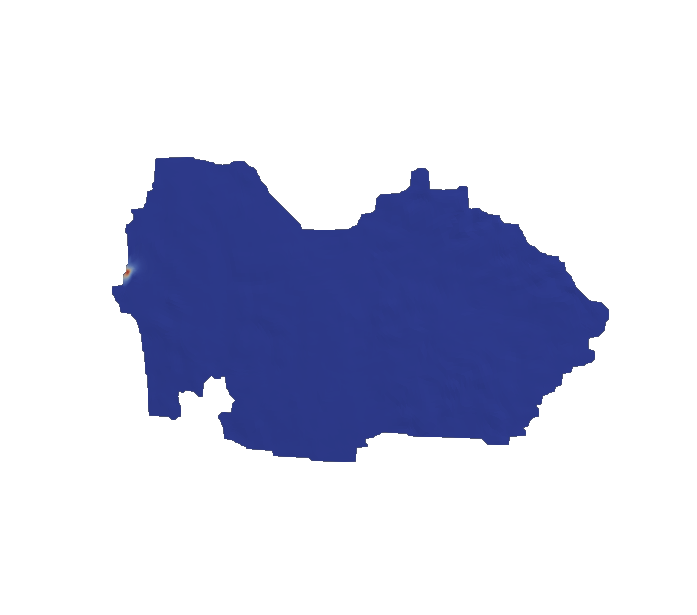
\includegraphics[width=1.0\columnwidth]{reordered_phi/phi8_minimal.png}
	\end{center}
}
	\only<10>{
	\begin{center}
		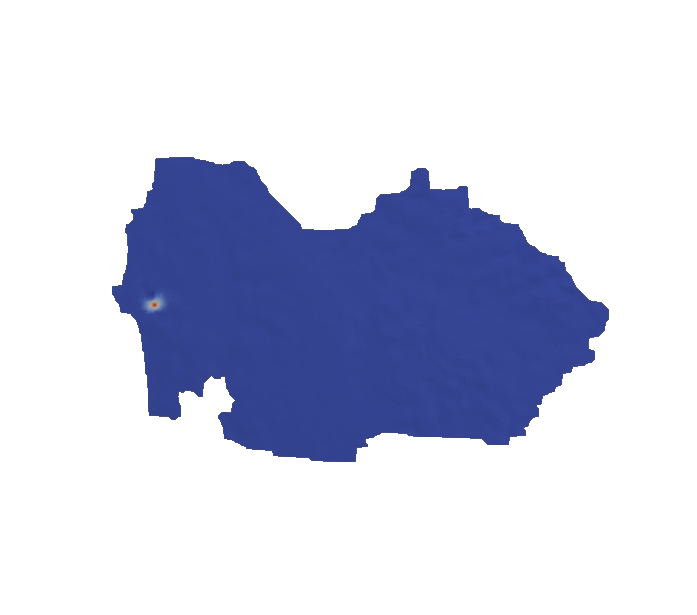
\includegraphics[width=1.0\columnwidth]{reordered_phi/phi9_minimal.png}
	\end{center}
}
	\only<11>{
	\begin{center}
		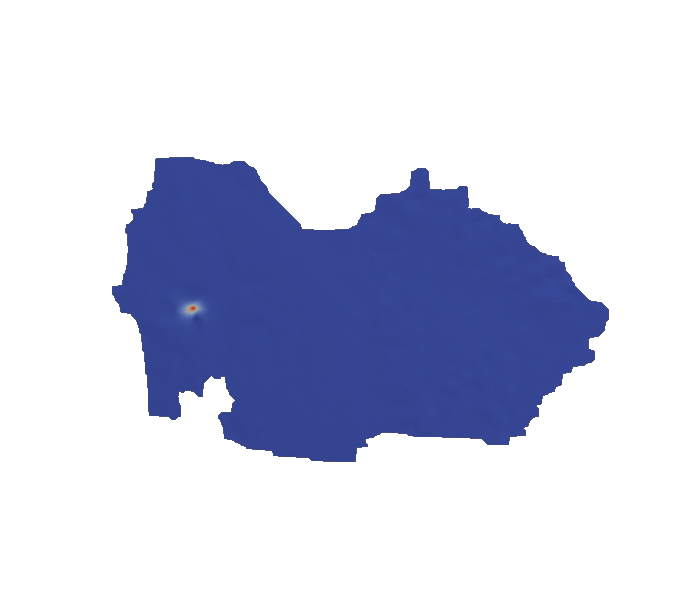
\includegraphics[width=1.0\columnwidth]{reordered_phi/phi10_minimal.png}
	\end{center}
}
	\only<12>{
	\begin{center}
		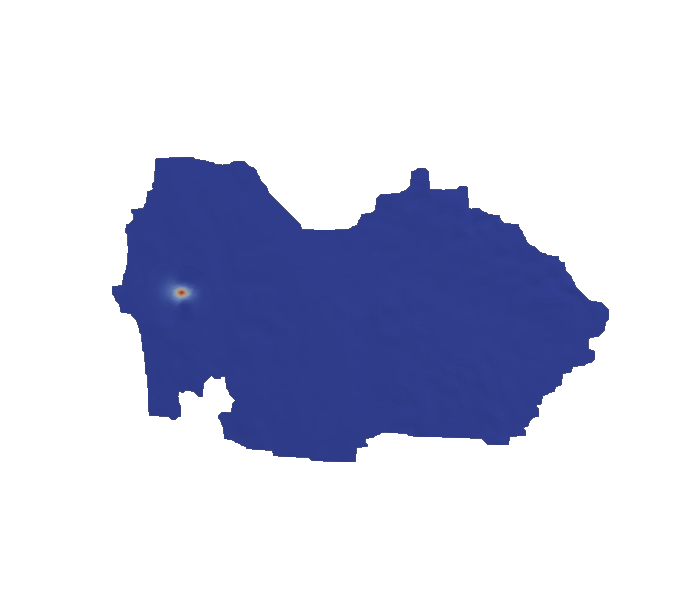
\includegraphics[width=1.0\columnwidth]{reordered_phi/phi11_minimal.png}
	\end{center}
}
	\only<13>{
	\begin{center}
		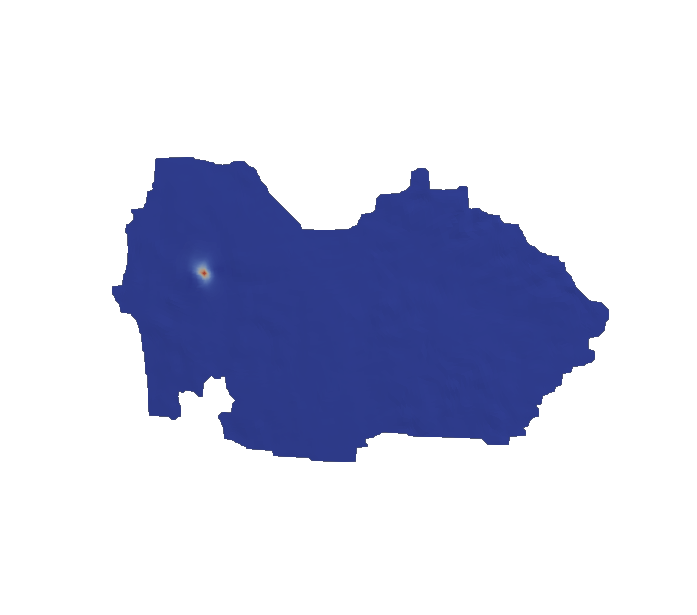
\includegraphics[width=1.0\columnwidth]{reordered_phi/phi12_minimal.png}
	\end{center}
}
	\only<14>{
	\begin{center}
		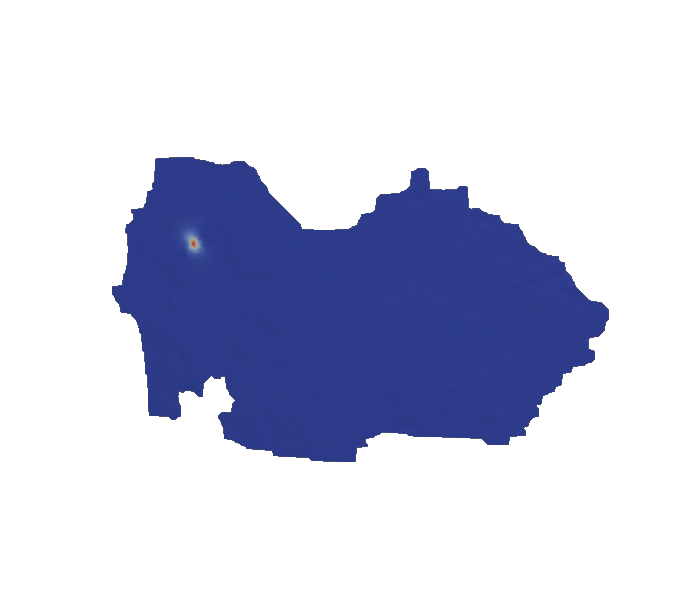
\includegraphics[width=1.0\columnwidth]{reordered_phi/phi13_minimal.png}
	\end{center}
}
	\only<15>{
	\begin{center}
		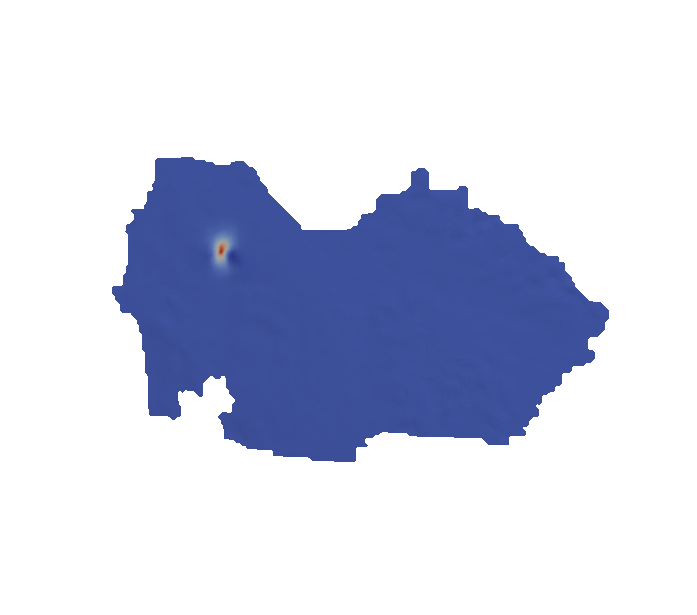
\includegraphics[width=1.0\columnwidth]{reordered_phi/phi14_minimal.png}
	\end{center}
}
	\only<16>{
	\begin{center}
		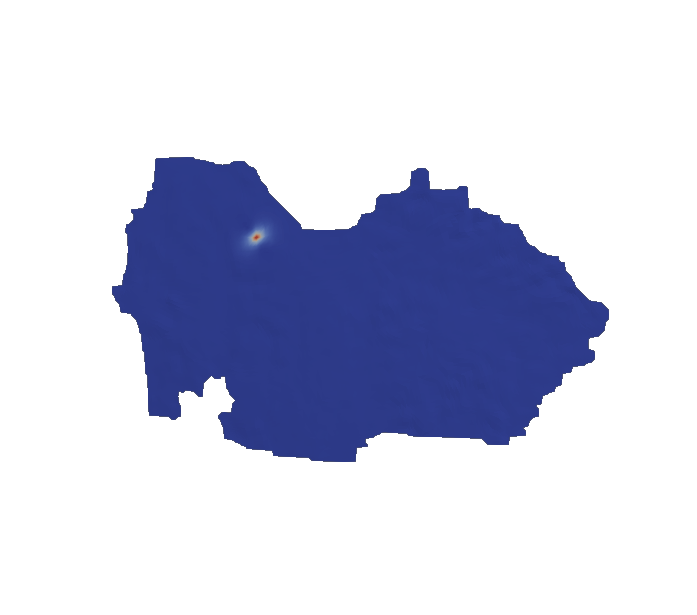
\includegraphics[width=1.0\columnwidth]{reordered_phi/phi15_minimal.png}
	\end{center}
}
	\only<17>{
	\begin{center}
		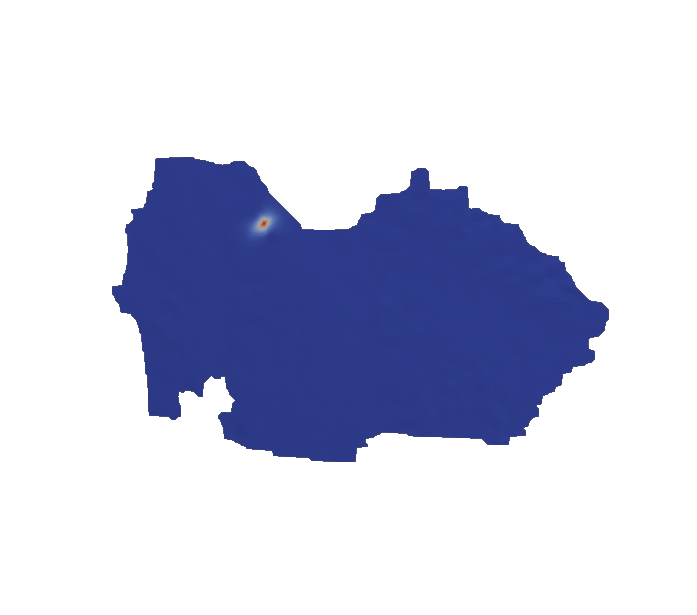
\includegraphics[width=1.0\columnwidth]{reordered_phi/phi16_minimal.png}
	\end{center}
}
	\only<18>{
	\begin{center}
		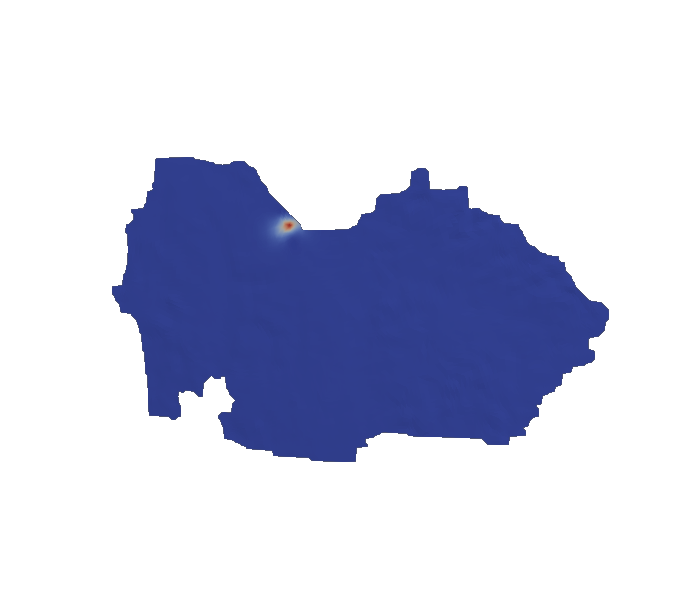
\includegraphics[width=1.0\columnwidth]{reordered_phi/phi17_minimal.png}
	\end{center}
}
	\only<19>{
	\begin{center}
		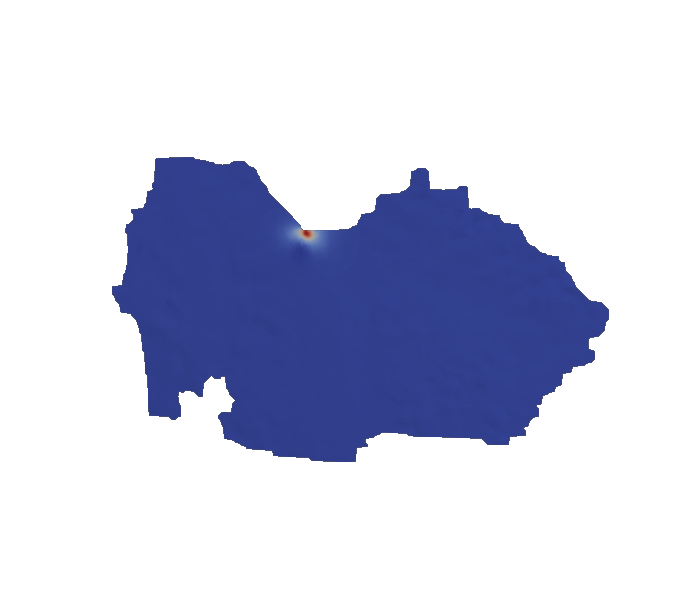
\includegraphics[width=1.0\columnwidth]{reordered_phi/phi18_minimal.png}
	\end{center}
}
	\only<20>{
	\begin{center}
		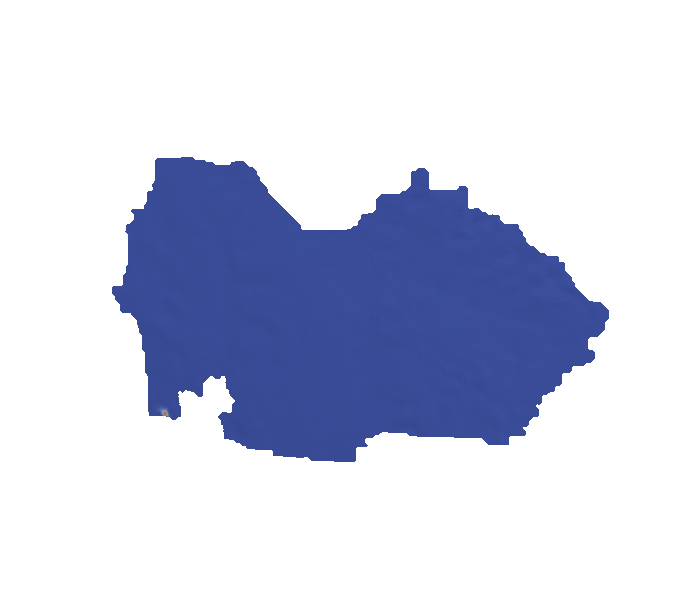
\includegraphics[width=1.0\columnwidth]{reordered_phi/phi19_minimal.png}
	\end{center}
}
	\only<21>{
	\begin{center}
		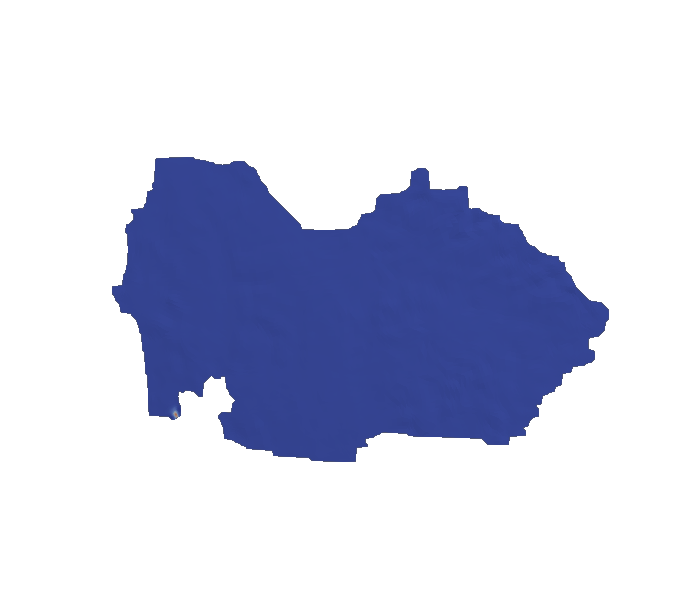
\includegraphics[width=1.0\columnwidth]{reordered_phi/phi20_minimal.png}
	\end{center}
}
	\only<22>{
	\begin{center}
		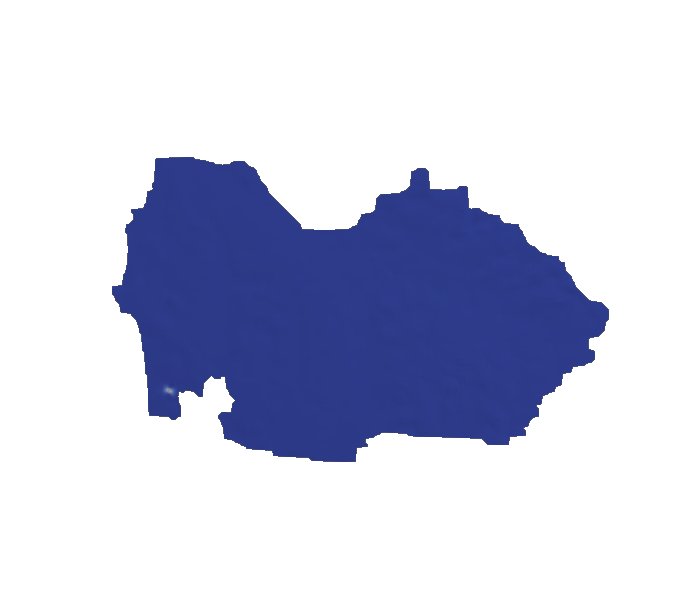
\includegraphics[width=1.0\columnwidth]{reordered_phi/phi21_minimal.png}
	\end{center}
}
	\only<23>{
	\begin{center}
		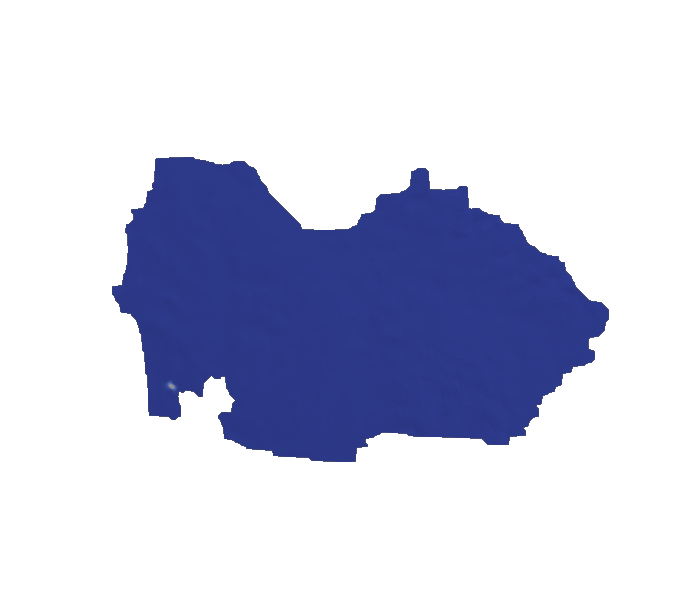
\includegraphics[width=1.0\columnwidth]{reordered_phi/phi22_minimal.png}
	\end{center}
}
	\only<24>{
	\begin{center}
		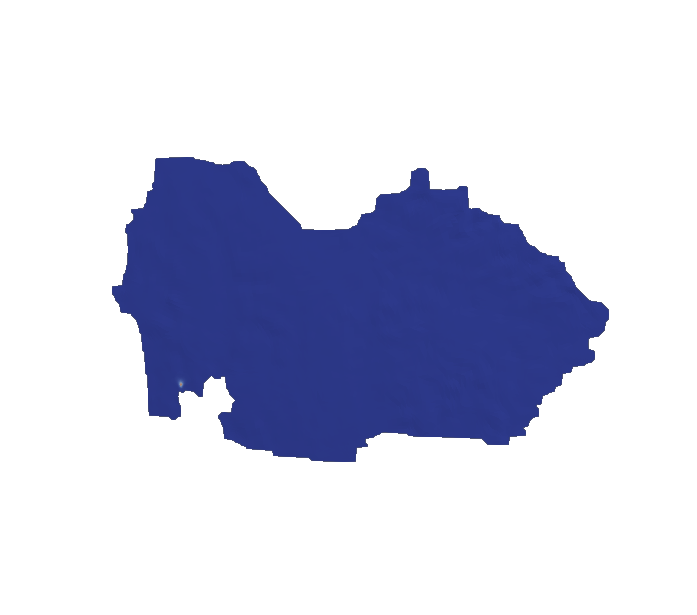
\includegraphics[width=1.0\columnwidth]{reordered_phi/phi23_minimal.png}
	\end{center}
}
	\only<25>{
	\begin{center}
		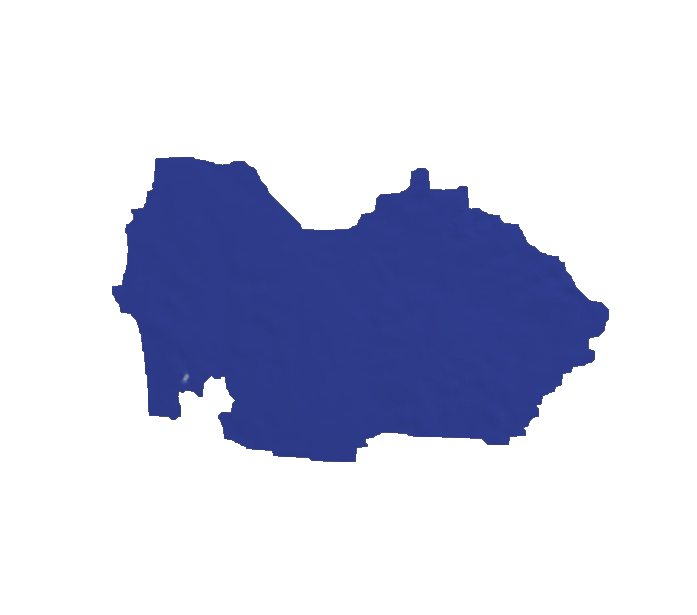
\includegraphics[width=1.0\columnwidth]{reordered_phi/phi24_minimal.png}
	\end{center}
}
	\only<26>{
	\begin{center}
		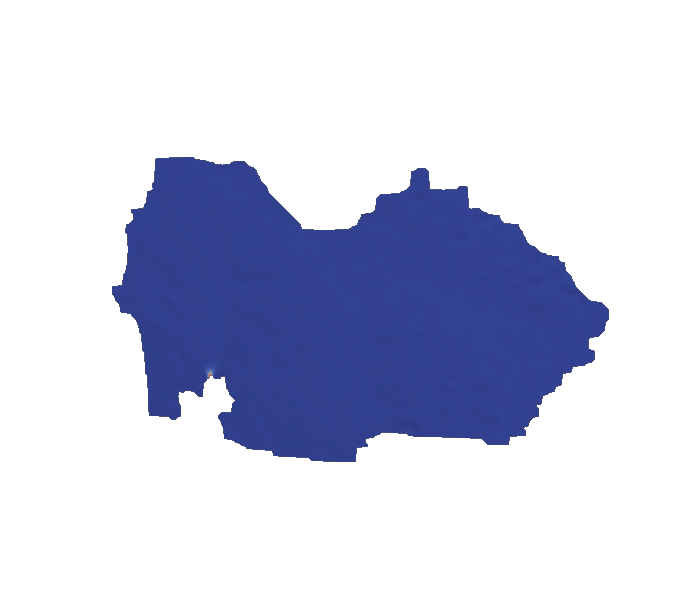
\includegraphics[width=1.0\columnwidth]{reordered_phi/phi25_minimal.png}
	\end{center}
}
	\only<27>{
	\begin{center}
		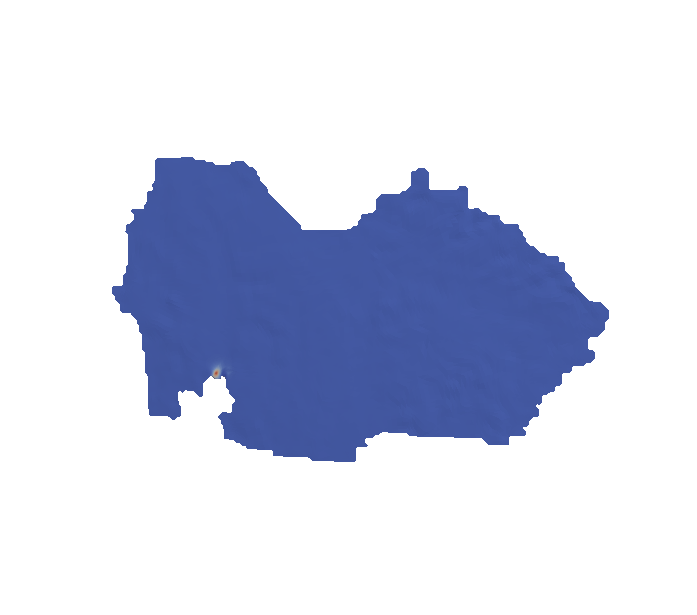
\includegraphics[width=1.0\columnwidth]{reordered_phi/phi26_minimal.png}
	\end{center}
}
	\only<28>{
	\begin{center}
		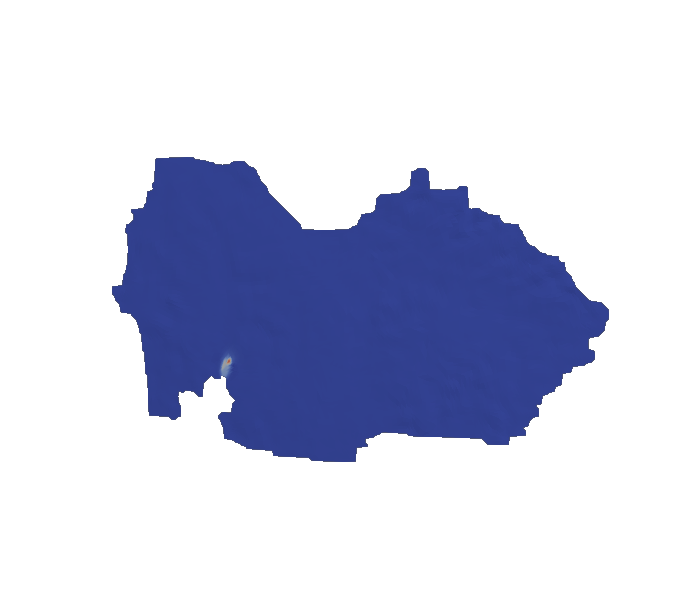
\includegraphics[width=1.0\columnwidth]{reordered_phi/phi27_minimal.png}
	\end{center}
}
	\only<29>{
	\begin{center}
		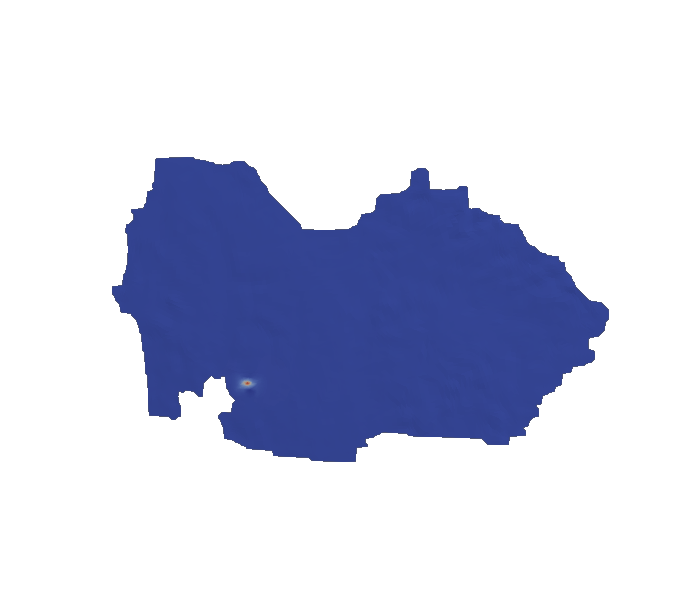
\includegraphics[width=1.0\columnwidth]{reordered_phi/phi28_minimal.png}
	\end{center}
}
	\only<30>{
	\begin{center}
		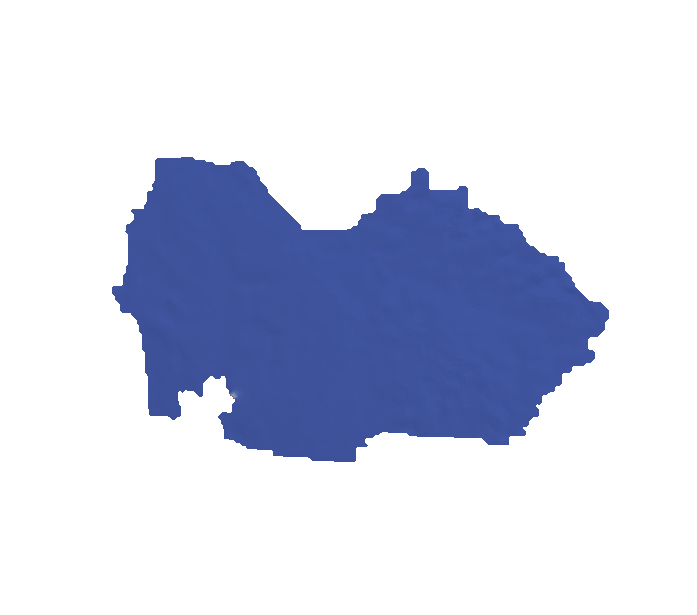
\includegraphics[width=1.0\columnwidth]{reordered_phi/phi29_minimal.png}
	\end{center}
}
	\only<31>{
	\begin{center}
		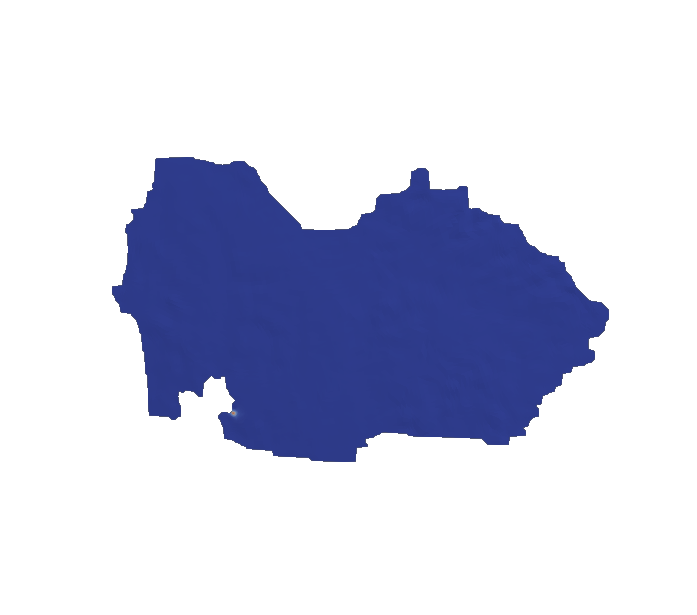
\includegraphics[width=1.0\columnwidth]{reordered_phi/phi30_minimal.png}
	\end{center}
}
	\only<32>{
	\begin{center}
		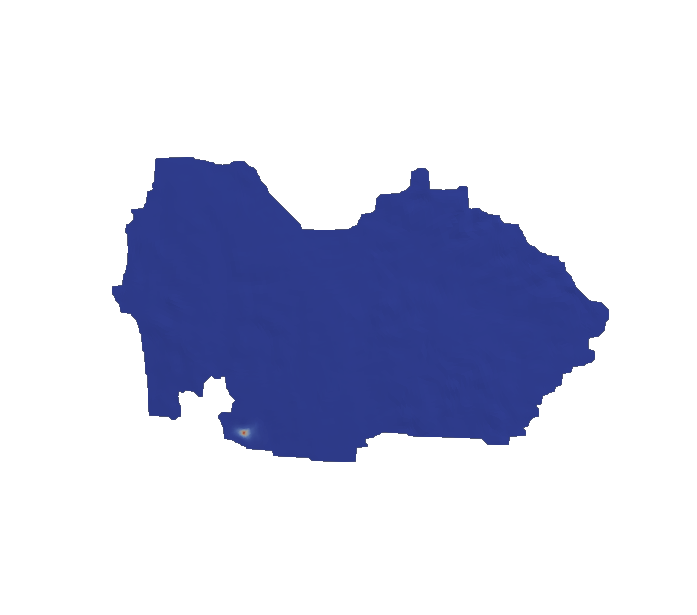
\includegraphics[width=1.0\columnwidth]{reordered_phi/phi31_minimal.png}
	\end{center}
}
	\only<33>{
	\begin{center}
		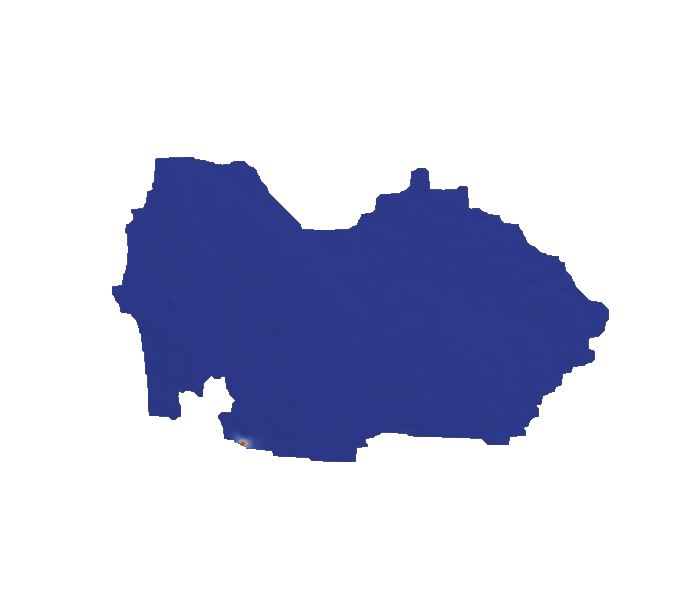
\includegraphics[width=1.0\columnwidth]{reordered_phi/phi32_minimal.png}
	\end{center}
}
	\only<34>{
	\begin{center}
		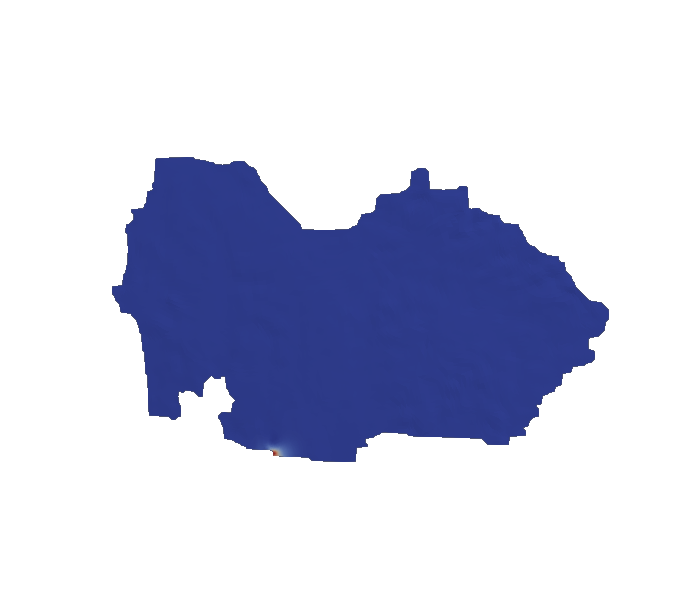
\includegraphics[width=1.0\columnwidth]{reordered_phi/phi33_minimal.png}
	\end{center}
}
	\only<35>{
	\begin{center}
		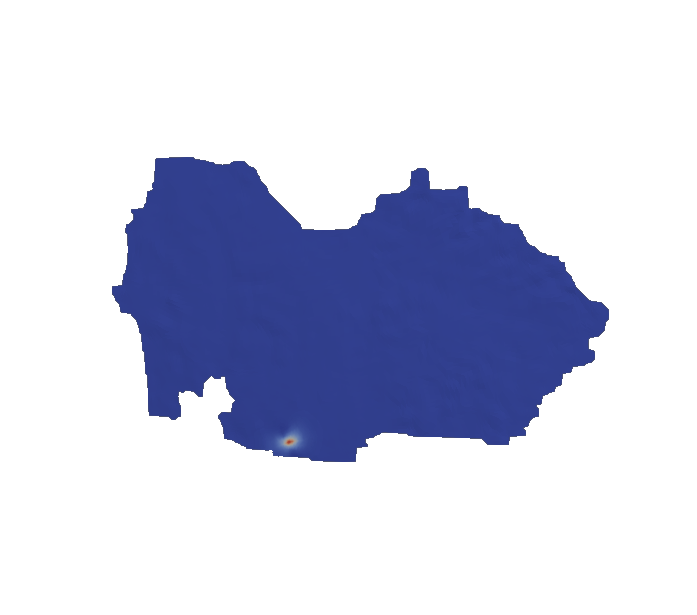
\includegraphics[width=1.0\columnwidth]{reordered_phi/phi34_minimal.png}
	\end{center}
}
	\only<36>{
	\begin{center}
		\includegraphics[width=1.0\columnwidth]{reordered_phi/phi35_minimal.png}
	\end{center}
}
	\only<37>{
	\begin{center}
		\includegraphics[width=1.0\columnwidth]{reordered_phi/phi36_minimal.png}
	\end{center}
}
	\only<38>{
	\begin{center}
		\includegraphics[width=1.0\columnwidth]{reordered_phi/phi37_minimal.png}
	\end{center}
}
	\only<39>{
	\begin{center}
		\includegraphics[width=1.0\columnwidth]{reordered_phi/phi38_minimal.png}
	\end{center}
}
	\only<40>{
	\begin{center}
		\includegraphics[width=1.0\columnwidth]{reordered_phi/phi39_minimal.png}
	\end{center}
}
	\only<41>{
	\begin{center}
		\includegraphics[width=1.0\columnwidth]{reordered_phi/phi40_minimal.png}
	\end{center}
}
	\only<42>{
	\begin{center}
		\includegraphics[width=1.0\columnwidth]{reordered_phi/phi41_minimal.png}
	\end{center}
}
	\only<43>{
	\begin{center}
		\includegraphics[width=1.0\columnwidth]{reordered_phi/phi42_minimal.png}
	\end{center}
}
	\only<44>{
	\begin{center}
		\includegraphics[width=1.0\columnwidth]{reordered_phi/phi43_minimal.png}
	\end{center}
}
	\only<45>{
	\begin{center}
		\includegraphics[width=1.0\columnwidth]{reordered_phi/phi44_minimal.png}
	\end{center}
}
	\only<46>{
	\begin{center}
		\includegraphics[width=1.0\columnwidth]{reordered_phi/phi45_minimal.png}
	\end{center}
}
	\only<47>{
	\begin{center}
		\includegraphics[width=1.0\columnwidth]{reordered_phi/phi46_minimal.png}
	\end{center}
}
	\only<48>{
	\begin{center}
		\includegraphics[width=1.0\columnwidth]{reordered_phi/phi47_minimal.png}
	\end{center}
}
	\only<49>{
	\begin{center}
		\includegraphics[width=1.0\columnwidth]{reordered_phi/phi48_minimal.png}
	\end{center}
}
	\only<50>{
	\begin{center}
		\includegraphics[width=1.0\columnwidth]{reordered_phi/phi49_minimal.png}
	\end{center}
}
	\only<51>{
	\begin{center}
		\includegraphics[width=1.0\columnwidth]{reordered_phi/phi50_minimal.png}
	\end{center}
}
	\only<52>{
	\begin{center}
		\includegraphics[width=1.0\columnwidth]{reordered_phi/phi51_minimal.png}
	\end{center}
}
	\only<53>{
	\begin{center}
		\includegraphics[width=1.0\columnwidth]{reordered_phi/phi52_minimal.png}
	\end{center}
}
	\only<54>{
	\begin{center}
		\includegraphics[width=1.0\columnwidth]{reordered_phi/phi53_minimal.png}
	\end{center}
}
	\only<55>{
	\begin{center}
		\includegraphics[width=1.0\columnwidth]{reordered_phi/phi54_minimal.png}
	\end{center}
}
	\only<56>{
	\begin{center}
		\includegraphics[width=1.0\columnwidth]{reordered_phi/phi55_minimal.png}
	\end{center}
}
	\only<57>{
	\begin{center}
		\includegraphics[width=1.0\columnwidth]{reordered_phi/phi56_minimal.png}
	\end{center}
}
	\only<58>{
	\begin{center}
		\includegraphics[width=1.0\columnwidth]{reordered_phi/phi57_minimal.png}
	\end{center}
}
	\only<59>{
	\begin{center}
		\includegraphics[width=1.0\columnwidth]{reordered_phi/phi58_minimal.png}
	\end{center}
}
	\only<60>{
	\begin{center}
		\includegraphics[width=1.0\columnwidth]{reordered_phi/phi59_minimal.png}
	\end{center}
}
	\only<61>{
	\begin{center}
		\includegraphics[width=1.0\columnwidth]{reordered_phi/phi60_minimal.png}
	\end{center}
}
	\only<62>{
	\begin{center}
		\includegraphics[width=1.0\columnwidth]{reordered_phi/phi61_minimal.png}
	\end{center}
}
	\only<63>{
	\begin{center}
		\includegraphics[width=1.0\columnwidth]{reordered_phi/phi62_minimal.png}
	\end{center}
}
	\only<64>{
	\begin{center}
		\includegraphics[width=1.0\columnwidth]{reordered_phi/phi63_minimal.png}
	\end{center}
}
	\only<65>{
	\begin{center}
		\includegraphics[width=1.0\columnwidth]{reordered_phi/phi64_minimal.png}
	\end{center}
}
	\only<66>{
	\begin{center}
		\includegraphics[width=1.0\columnwidth]{reordered_phi/phi65_minimal.png}
	\end{center}
}
	\only<67>{
	\begin{center}
		\includegraphics[width=1.0\columnwidth]{reordered_phi/phi66_minimal.png}
	\end{center}
}
	\only<68>{
	\begin{center}
		\includegraphics[width=1.0\columnwidth]{reordered_phi/phi67_minimal.png}
	\end{center}
}
	\only<69>{
	\begin{center}
		\includegraphics[width=1.0\columnwidth]{reordered_phi/phi68_minimal.png}
	\end{center}
}

\end{frame}
%---------------------------------------------------------------------------------%
\begin{frame}
  \frametitle{Hessian approximation method: big idea}
      \begin{itemize}
      \item {\bf Step 1:} Compute ``batches'' of impulse responses by applying Hessian to Dirac combs
      \item {\bf Step 2:} Interpolate known impulse responses to approximate unknown Hessian entries $\mathbf{H}_{ij}$
      \item {\bf Step 3:} Convert to $\mathcal{H}$-matrix to do linear algebra
      \end{itemize}
  	\includegraphics[width=0.45\columnwidth]{impulse_batch1.png}  \includegraphics[width=0.45\columnwidth]{impulse_batch2.png}
  *Impulse response batches from Ice Mountain
\end{frame}
%---------------------------------------------------------------------------------%
%---------------------------------------------------------------------------------%
\begin{frame}
	\frametitle{Technical details}
	{\Large
		\begin{itemize}
			\setlength\itemsep{2em}
			\item How do we choose the impulse response points?
			\begin{itemize}
				\item {\large How do we make sure they don't overlap?}
			\end{itemize}
			\item How do we interpolate the impulse responses? 
			\begin{itemize}
				\item {\large What about boundary issues?}
			\end{itemize}
		\end{itemize}
	}
\end{frame}
%---------------------------------------------------------------------------------%
\begin{frame}
	\frametitle{How to choose impulse response points?}
	One hessian matrix-vector product $\rightarrow$ many impulse responses
	\begin{center}
		\includegraphics[width=0.5\columnwidth]{impulse_batch2.png} 
	\end{center}
	\begin{itemize}
		\item \textbf{Goal:} choose as many points as possible, such that the impulse response supports don't overlap
		\item \textbf{Dilemma:} How can we know the impulse response supports before we compute them?
	\end{itemize}
\end{frame}
%---------------------------------------------------------------------------------%
\begin{frame}
	\frametitle{Matrix analogy: getting all row sums}
	
	\textbf{Matrix:} let $\mathbf{A} \in \mathbb{R}^{N \times N}$. Then
	
	$$\mathbf{A}^T \begin{bmatrix}
	1 \\ 1 \\ \vdots \\ 1
	\end{bmatrix} = \begin{bmatrix}
	\text{sum of }\mathbf{A} \text{ col }1 \\
	\text{sum of }\mathbf{A} \text{ col }2 \\
	\vdots \\
	\text{sum of }\mathbf{A} \text{ col }N
	\end{bmatrix}$$
	
	Apply matrix to vector of ones $\rightarrow$ get row sums for all rows
	
	\vspace{3em}
	
	\textbf{Operator:} let $C(x)=1$ be the constant function. Then 
	
	$$(H_d^T C)^*(y) = \int_\Omega \left(H_d \delta_y\right)(x) dx$$
	
	
	Apply Hessian to constant function $\rightarrow$ get volumes of every impulse response
\end{frame}
%---------------------------------------------------------------------------------%
\begin{frame}
	\frametitle{Mean and standard deviations of impulse responses}
	\begin{itemize}
		\setlength\itemsep{2em}
		\item Let $V(x)$, $\mu(x)$, and $\Sigma(x)$ be the ``volume'', ``mean'', and ``variance'' of $\phi_x$
		\item Let $C$, $L^i$, and $Q^{ij}$ be the following functions:
		\begin{equation*}
		C(x) := 1, \qquad
		L^i(x) := x^i, \qquad
		Q^{ij}(x) = x^i x^j
		\end{equation*}
		\item Then
		\begin{align*}
		V =& \left(H_d^T C\right)^* \\
		\mu^i =& \left(H_d^T L^i\right)^* / V \\
		\Sigma^{ij} =& \left(H_d^T Q^{ij}\right)^* / V - \mu^i\cdot \mu^j
		\end{align*}
		\item Apply Hessian to constant, linear, and quadratic functions $\rightarrow$ get estimates of support for every impulse response
	\end{itemize}
	
\end{frame}

\begin{frame}
	\frametitle{Impulse response moments}
	$\phi_x$ is \textbf{approximately supported} in the ellipsoid:
	$$E = \{y: (y - \mu(x))^T\Sigma(x)^{-1}(y - \mu(x)) \le \tau^2\}$$
	\begin{center}
		\includegraphics[scale=0.28]{frog_moments4.pdf}
	\end{center}
\end{frame}
%---------------------------------------------------------------------------------%
\begin{frame}
	\frametitle{Impulse response batches via ellipsoid packing}
	\begin{itemize}	
		\setlength{\itemsep}{1em}
		\item Picking impulse response points becomes an \textbf{ellipsoid packing problem}
		\item Pack ellipsoids using \textbf{greedy algorithm}
		\item Get batch of impulse responses by applying Hessian to \textbf{Dirac comb} (weighted sum of delta functions associated with ellipsoids)
		\item \textbf{Repeat} to get more batches
	\end{itemize}
	\vspace{2em}
  	\includegraphics[width=0.9\columnwidth]{frog_batches3.pdf}  
\end{frame}


\begin{frame}
	\frametitle{Radial basis function interpolation}
	\begin{center}
%		\includegraphics[width=0.8\textwidth]{interpolation_rbf.pdf}
 	\includegraphics[width=1.0\columnwidth]{frog_hmatrix_knn_impulse3.pdf}
	\end{center}
	\begin{itemize}
		\item Must compute $O(N \log N)$ kernel entries $\Phi(y,x)$ to construct H-matrix
		\item For each entry, interpolate impulse responses using radial basis functions.
		\item Use only $k$-nearest neighbors (must solve $k \times k$ linear system)
	\end{itemize}
\end{frame}

\begin{frame}
	\frametitle{Computational cost}
	\begin{itemize}
	  	\setlength\itemsep{2em}
		\item \textbf{Hessian-vector products:} 
		$$6 + n_\text{batches}$$
		E.g., $11$ Hessian-vector products for $5$ batches of impulse responses
		\item \textbf{Ellipsoid intersection tests:}
		$$O(Nm)$$
		where $m$ is total number of impulse responses in all batches
		\item \textbf{Elementary operations} to build and use the H-matrix:
		$$O(N \log N)$$ 
	\end{itemize}
\end{frame}


%---------------------------------------------------------------------------------%

%\begin{frame}
%	\frametitle{Boundary considerations (1)}
%	\begin{center}
%		\includegraphics[width=0.8\textwidth]{interpolation_rbf_boundary.pdf}
%	\end{center}
%	\begin{itemize}
%		\item If $p_i + y - x$ is outside the domain, don't use $i$th impulse response for $H(y,x)$
%	\end{itemize}
%\end{frame}
%---------------------------------------------------------------------------------%

%\begin{frame}
%	\frametitle{Boundary considerations (2)}
%	\begin{center}
%		\includegraphics[width=0.8\textwidth]{interpolation_rbf_adjoint.pdf}
%	\end{center}
%	\begin{itemize}
%		\item Take advantage of symmetry
%	\end{itemize}
%\end{frame}
%---------------------------------------------------------------------------------%

%---------------------------------------------------------------------------------%
%\begin{frame}
%	\frametitle{How to choose impulse response points?}
%	One hessian matrix-vector product $\rightarrow$ many impulse responses
%	\begin{center}
%		\includegraphics[width=0.5\columnwidth]{IRB1.png} 
%	\end{center}
%	\begin{itemize}
%		\item \textbf{Goal:} choose as many points as possible, such that the impulse response supports don't overlap
%		\item \textbf{Dilemma:} How can we know the impulse response supports before we compute them?
%	\end{itemize}
%\end{frame}
%---------------------------------------------------------------------------------%

%---------------------------------------------------------------------------------%

%---------------------------------------------------------------------------------%

%---------------------------------------------------------------------------------%
\begin{frame}
	\frametitle{Ice Mountain: Setup}
	\begin{figure}
		\begin{center} 
			\begin{subfigure}{0.99\textwidth}
				\begin{center} 
					\includegraphics[scale=0.2]{meshHeight_view2_edges.png}
				\end{center}
				\caption{Ice sheet model geometry}
				\label{fig:ice_mountain_mesh}
			\end{subfigure} \\
			\begin{subfigure}{0.49\textwidth}
				\includegraphics[scale=0.2]{mtrue_withColorBar.png}
				\caption{$\beta_\text{true}$}
				\label{fig:true_beta}
			\end{subfigure}
			\begin{subfigure}{0.49\textwidth}
				\includegraphics[scale=0.2]{trueVelocity2_glyphs.png}
				\caption{$v_\text{true}$}
				\label{fig:stokes_velocity}
			\end{subfigure}
		\end{center}
	\end{figure} 
\end{frame}

%---------------------------------------------------------------------------------%
\begin{frame}
	\frametitle{Ice Mountain: Reconstructions}
\begin{figure}
	\begin{subfigure}{0.32\textwidth}
		\includegraphics[scale=0.17]{mstar_0.25noise_cropped.png}
		\caption{25\% noise}
	\end{subfigure}
	\begin{subfigure}{0.32\textwidth}
		\includegraphics[scale=0.17]{mstar_0.05noise_cropped.png}
		\caption{5\% noise}
	\end{subfigure}
	\begin{subfigure}{0.32\textwidth}
		\includegraphics[scale=0.17]{mstar_0.01noise_cropped.png}
		\caption{1\% noise}
	\end{subfigure}
%	\caption{(Ice sheet) The log basal friction parameter, with color scale as in Figure~\ref{fig:true_beta}, computed from the PDE constrained optimization problem with noise levels: $25\%$ (left), $5.0\%$ (middle), and $1.0\%$ (right).}
%	\label{fig:stokes_reconstructions} 
\end{figure}
\begin{itemize}
\item Deterministic reconstruction / MAP point for varying noise levels
\item Bi-Laplacian regularization / prior
\item Regularization / ``prior'' strength chosen via Morozov discrepancy principle
\end{itemize}
\end{frame}

\begin{frame}
\frametitle{Ice Mountain: inexact Newton-CG convergence}
\begin{itemize}
	\item 5\% noise
	\item Preconditioner build at 3rd Newton iteration and re-used for all subsequent iterations
	\item PSF (5): our preconditioner with 5 batches.
	\item REG: regularization preconditioning.
	\item NONE: no preconditioning.
\end{itemize}
\vspace{0.5em}
	{\footnotesize
	\begin{center}
		\begingroup
		\setlength{\tabcolsep}{3pt}
		\renewcommand{\arraystretch}{1.1}
		\begin{tabular}{c| c c c | c c c | c c c}
			&  \multicolumn{3}{|c|}{PSF (5)} & \multicolumn{3}{|c|}{REG} & \multicolumn{3}{|c}{NONE} \\
			\hline
			Iter & 
			\#CG & \#Stokes & $\|\mathbf{g}\|$ & 
			\#CG & \#Stokes & $\|\mathbf{g}\|$ & 
			\#CG & \#Stokes & $\|\mathbf{g}\|$ \\
			0 &
			1 & 4 & 1.9e+7 &
			3 & 8 & 1.9e+7 &
			1 & 4 & 1.9e+7 \\
			1 &
			2 & 6  & 6.1e+6 &
			8 & 18 & 8.4e+6 &
			2 & 6  & 6.1e+6 \\
			2 &
			4 & 10 & 2.6e+6 &
			16 & 34 & 4.1e+6 &
			4 & 10 & 2.6e+6 \\
			3 &
			2 & 6+22 & 6.9e+5 &
			34 & 70 & 1.8e+6 &
			14 & 30 & 6.9e+5 \\
			4 &
			3 & 8 & 4.4e+4 &
			52 & 106 & 5.6e+5 &
			29 & 60 & 1.3e+5 \\
			5 &
			5 & 12 & 2.2e+3 &
			79 & 160 & 9.4e+4 &
			38 & 78 & 1.0e+4 \\
			6 &
			0 & 2 & 1.1e+1 &
			102 & 206 & 6.5e+3 &
			58 & 118 & 1.8e+2 \\
			7 &
			--- & --- & --- &
			151 & 304 & 1.2e+2 &
			0 & 2 & 5.5e-1 \\
			8 & 
			--- & --- & --- &
			0 & 2 & 2.9e-1 &
			--- & --- & --- \\
			\hline
			Total & 
			17 & 70 & --- &
			445 & 908 & --- &
			146 & 308 & --- \\
		\end{tabular}
		\endgroup
	\end{center}
}
\end{frame}

\begin{frame}
	\frametitle{Ice Mountain: preconditioned Hessian spectral properties}
\begin{figure}
	\begin{subfigure}{0.53\textwidth}
		\centering
		\includegraphics[scale=0.9]{stokes_pcg_convergence.pdf}
	\end{subfigure}
	\begin{subfigure}{0.46\textwidth}
		\begin{center}
			\includegraphics[scale=0.9]{stokes_geigs_figure.pdf}
		\end{center}
	\end{subfigure}
\end{figure} 
	\begin{itemize}
		\item Hessian evaluated at MAP point for 5\% noise.
		\item Left: solving $\mathbf{H}\mathbf{x}=-\mathbf{b}$ via preconditioned conjugate gradient
		\item Right: eigenvalues for generalized eigenvalue problem $\mathbf{H}\mathbf{u}=\lambda \widetilde{\mathbf{H}}\mathbf{u}$
	\end{itemize}
\end{frame}

\begin{frame}
	\frametitle{Ice Mountain: preconditioned Hessian condition number}
		\begin{center}
		{\large
			\begingroup
			\setlength{\tabcolsep}{4pt}
			\renewcommand{\arraystretch}{1.25}
			\begin{tabular}{c| c c c c c}
				noise    & \multicolumn{5}{c}{COND$(\widetilde{\mathbf{H}}^{-1} \mathbf{H})$ } \\ \cline{2-6}
				level    & REG     &	NONE  & PSF $(1)$ & PSF $(5)$ & PSF $(25)$ \\ \hline 
				$25\%$   & 1.01e+3 & 2.96e+3  & 1.34e+0   & 1.30e+0   & 1.18e+0    \\ 
				$11\%$   & 7.40e+3 & 1.05e+3  & 2.27e+0   & 1.55e+0   & 1.31e+0    \\   
				$5.0\%$  & 3.29e+4 & 4.96e+2  & 5.61e+0   & 3.06e+0   & 1.92e+0    \\ 
				$2.2\%$  & 1.66e+5 & 8.89e+2  & 1.58e+1   & 8.07e+0   & 4.03e+0    \\  
				$1.0\%$  & 5.36e+5 & 1.61e+3  & 7.17e+1   & 1.93e+1   & 9.19e+0    \\   
			\end{tabular}
			\endgroup
		}
	\end{center}
\end{frame}

%---------------------------------------------------------------------------------%

%---------------------------------------------------------------------------------%

%---------------------------------------------------------------------------------%

%---------------------------------------------------------------------------------%

%--------------------------------------------------------------------------
\begin{frame}
  \frametitle{Summary}

  \begin{itemize}
  	\setlength\itemsep{1.5em}
  \item Hessian approximations or preconditioners are essential for solution of Bayesian inverse problems governed by
    partial differential equations.
    \vspace{0.05in}
  \item Low-rank approximations of the Hessian become
    prohibitive as the data becomes more informative, as is the case
    for ice sheet inverse problems.
    \vspace{0.05in}
  \item Local point spread function interpolation combined with Hierarchical matrix representations promise a more efficient
    Hessian approximation.
  \end{itemize}
	\vspace{2em}
	{\small Alger, N., Hartland, T., Petra, N., Ghattas, O. (2023). Point spread function approximation of high rank Hessians with locally supported non-negative integral kernels. To appear in SISC.}
\end{frame}


\end{document}
